\pgfplotsset{
    standard/.style={
        axis x line=middle,
        axis y line=middle,
        enlarge x limits=0.15,
        enlarge y limits=0.15,
        every axis x label/.style={
            at={(current axis.right of origin)},
            anchor=north west
        },
        every axis y label/.style={
            at={(current axis.above origin)},
            anchor=north east
        },
        every axis plot post/.style={
            mark options={fill=white}
        },
    },
    wideybar/.style={
        standard,
        ybar,
        enlargelimits=0.15,
        axis y line=left,
        ymin=0,
        scale only axis, % apply height and width to the actual axis
        height=5cm,
        % width=\textwidth-\widthof{100}-0.1cm, % textwidth - the longest label offset; does not work for some reason
        width=15.5cm,
        % yticklabel style={align=right, inner sep=0pt, xshift=-0.1cm}, % does not work for some reason
    },
}
\definecolor{backcolor}{rgb}{0.95,0.95,0.92}
\definecolor{codegreen}{rgb}{0,0.6,0}
\definecolor{codegreen2}{rgb}{0,0.6,0.2}
\definecolor{codepurple}{rgb}{0.6,0,0.6}
\definecolor{codeorange}{rgb}{0.8,0.2,0}
\lstdefinestyle{mystyle}{%
    showspaces=false,
    showtabs=false,
    breaklines=true,
    showstringspaces=false,
    breakatwhitespace=true,
    escapeinside={(*@}{@*)},
    backgroundcolor=\color{backcolor},
    commentstyle=\color{codegreen},
    keywordstyle=\color{codepurple},
    keywordstyle=[2]\color{darkblue},
    keywordstyle=[3]\color{codepurple},
    keywordstyle=[4]\color{codegreen2},
    stringstyle=\color{codeorange},
    basicstyle=\ttfamily,
    captionpos=b,
    numbers=left,
    frame=single,
    numberstyle=\tiny,
    aboveskip=1em,
    abovecaptionskip=6pt,
}%
\lstset{style=mystyle}%
\lstdefinelanguage{PythonPlus}[]{Python}{%
    morekeywords=[1]{,as,assert,nonlocal,with,yield},
    morekeywords=[2]{,self,True,False,None,},
    morekeywords=[4]{,ValueError},
}%

\chapter{Úvod}
\label{cha:introduction}

Steganografie je obor zabývající se skrýváním informace takovým způsobem, aby
nebylo možné zjistit její přítomnost. Důvod pro takovéto skrývání informace
může být zajištění bezpečnosti před třetí stranou, pro kterou není informace
určena. Steganografie se dnes dělí na tradiční a~digitální. V~digitální
steganografii je velké množství typů dat, do kterých je možné vkládat utajované
informace a~digitální zvuk je jedním z~nich.

V~oblasti digitální zvukové steganografie je dostupné velké množství kvalitní
literatury popisující teoretické fungování metod, kterými se jednotlivé
publikace zabývají. Je však těžké najít konkrétní implementace popisovaných
metod i~přesto, že autoři je implementovali pro získání výsledků. Proto je
hlavním cílem této práce vytvořit softwarovou knihovnu a~program
v~programovacím jazyce Python, aby měl kdokoliv možnost pracovat na výzkumu
v~této vědecké disciplíně. Ne vždy stačí pouze algoritmický popis různých metod
pro pochopení jejich fungování. Implementace v~konkrétním programovacím jazyce
nám přináší formalismus, který umožňuje snazší pochopení. Chtěl bych proto
touto prací přispět v~této oblasti tím, že bude přístupnější pro širší
veřejnost.

V~následujících kapitolách této práce je shrnut současný stav tohoto oboru,
jsou vysvětleny cíle a~technické prostředky použité k~jejich dosažení
a~zhodnoceny dosažené výsledky. V~kapitole~\ref{cha:digital-steganography} jsou
do hloubky popsány steganografické metody vybrané pro implementaci a~některé
další používané. Kapitola~\ref{cha:library-design} popisuje, proč byl vybrán
programovací jazyk Python a~použité knihovny. Je zde také popsána struktura
balíčků pro Python a~steganografické metody, které byly vybrány pro
implementaci. Na konci kapitoly je popsán způsob vyhodnocení kvality metod
a~popis vlastní metody. Kapitola~\ref{cha:implementation} je zaměřená na popis
rozvržení kódu a~implementaci steganografických metod.
Kapitola~\ref{cha:method-evaluation} obsahuje výsledky testování a~srovnání
metod. Na závěr obsahuje kapitola~\ref{cha:conclusion} shrnutí výsledků práce
a~vyhlídky do budoucna.

Text této práce je dostupný pod licencí
CC-BY-4.0\footnote{\url{https://creativecommons.org/licenses/by/4.0}} na adrese
\url{https://github.com/pkabelka/audio-steganography-thesis}.


\chapter{Digitální steganografie}
\label{cha:digital-steganography}

Tato kapitola představí steganografii obecně a~její klasifikace. Poté bude
stručně popsán způsob, jakým se dnes reprezentuje digitální zvuk. Dále budou
vysvětleny vlastnosti, na základě kterých budou metody hodnoceny a~srovnávány
včetně způsobu jejich ověření. Zbytek této kapitoly se bude věnovat existujícím
steganografickým metodám včetně jejich možných modifikací.

\section{Základní definice a~klasifikace}
\label{sec:definitions}

Steganografie je praktika skrývání informace s~cílem zakrýt její samotnou
existenci a~ne jen znemožnit její čtení
\cite{AlSabhany2020}\cite{Anderson1998}\cite{Djebbar2012}\cite{Dutta2020}.
Původ této praktiky se vrací až do antiky -- vyrytím písma do destičky, která
se následně zalila voskem; ve středověké Evropě položením papíru nebo dřevěné
šablony na nevinně vypadající text, čímž zvýrazní tajnou zprávu. Steganografie
se tedy v~různých podobách praktikovala po tisíciletí až do dnešní počítačové
doby~\cite{Anderson1998}, kdy je považována za podobor zabezpečení dat
\cite{Djebbar2012} a~více se přesouvá od tradiční k~digitální steganografii.

V~dnešním světě se stalo zabezpečení dat zájmem všech a~steganografie jako
proces ukrývání zprávy do jiného typu média slouží k~ochraně před
neautorizovanými či neoprávněnými příjemci~\cite{Dutta2020}. Médium, do kterého
je informace skrývána, se nazývá nosič a~může být různých typů, jako například
obrázek, audio, video, IP datagram~\cite{Dutta2020}, text a~mnoho dalších.
Hierarchickou klasifikaci je možné vidět na obrázku
\ref{pic:steganography-classification}.

\begin{figure}[hbt]
    \centering
    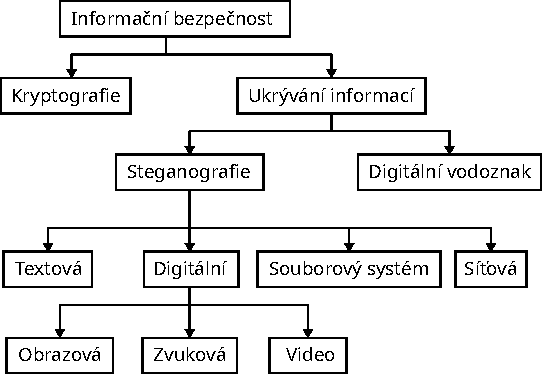
\includegraphics[width=0.8\textwidth]{obrazky/steganography-classification.pdf}
    \caption{Klasifikace oboru informační bezpečnosti a~steganografie.
    Přeloženo z~\cite{Majeed2021}.}
    \label{pic:steganography-classification}
\end{figure}

Pokud je nosičem počítačový soubor, pak se může nazývat \textit{krycí soubor}.
Názvy \textit{nosič} a~\textit{krycí soubor} jsou však často zaměnitelné. Každý
typ nosiče má svoji oblast výzkumu, která se jej týká. Některé steganografické
metody používané u~různých typů nosičů jsou konceptuálně stejné a~v~praxi se
aplikují podobným způsobem. Tato práce se však bude zabývat pouze metodami
použitelnými pro digitální zvuk a~proto následující podkapitola vysvětlí
způsob, jakým se zvuk reprezentuje v~digitální formě.

\section{Reprezentace a~způsob uložení digitálního zvuku}
\label{sec:digital-sound-representation}

V~reálném světě se zvuk vyskytuje jako vibrace materiálu při frekvenci
slyšitelné člověkem, která se pohybuje mezi 10\,Hz a~20\,000\,Hz
\cite{Swanson1998}. Zvuk je ve skutečném světě spojitý signál -- má nekonečný
počet hodnot -- a~je tedy definován všude. Základními parametry signálu jsou
\textit{frekvence}, \textit{perioda} a~\textit{amplituda}. Amplituda udává
maximální výchylku signálu. Frekvence, nebo také kmitočet, vyjadřuje počet
period za jednotku času a~udává se v~Hertzích (Hz). Perioda je úzce svázaná
s~frekvencí a~vyjadřuje délku jednoho opakování v~signálu, udává se
v~sekundách~\cite{Cernocky2021}. Vztah mezi frekvencí a~periodou lze vidět
v~rovnici~\ref{eq:period}, kde $T$~je perioda a~$f$~je frekvence.

\begin{equation}
    \label{eq:period}
    T = \frac{1}{f}
\end{equation}

Aby bylo možné se zvukem pracovat
digitálně, je nutné jej převést do diskrétní formy, která má konečný počet
hodnot. Toho je možné docílit vzorkováním signálu na určité vzorkovací
frekvenci a~poté kvantováním~\cite{Cernocky2021}. Posledním krokem pro převod
spojitého signálu na digitální je kódování. Tyto tři procesy tvoří systém,
který se nazývá \textit{pulzně-kódová modulace}~(PCM)~\cite{Oliver1948}, který
je neopominutelným základem pro práci s~digitálním audiem.

\subsection*{Vzorkování}
\label{sub:sampling}

Vzorkování probíhá tak, že se každá sekunda spojitého signálu rozdělí na tolik
bodů, kolik udává vzorkovací frekvence. V~každém bodě se zjistí amplituda ve
stejném bodě spojitého signálu a~ta se stane jeho hodnotou. Rozdíl mezi
spojitým a~navzorkovaným signálem je vidět na
obrázku~\ref{pic:continuous-vs-sampled-signal}. Aby nedošlo ke ztrátě
informace, je nutné dodržet Nyquist-Shannonův vzorkovací teorém, podle kterého
musí být nejvyšší frekvence přítomná v~signálu maximálně polovina vzorkovací
frekvence~\cite{Shannon1949}. Nejčastěji používané vzorkovací frekvence jsou
44\,100\,Hz a~48\,000\,Hz. Nejvyšší frekvence, které lze na těchto vzorkovacích
frekvencích reprezentovat bez ztráty informace jsou příslušně 22\,050\,Hz
a~24\,000\,Hz.

\begin{figure}[hbt]
    \centering
    \begin{subfigure}[b]{0.5\linewidth}
        \centering
        \begin{tikzpicture}
            \begin{axis}[%
                standard,
                scale=0.9,
                domain=0:1,
                samples=100,
                xlabel={$t~[s]$},
                ylabel={$x(t)$},
                ylabel style={yshift=10pt},
                ]
                \addplot[blue,thick] {sin(2*180*x)};
            \end{axis}
        \end{tikzpicture}
    \end{subfigure}%
    \begin{subfigure}[b]{0.5\linewidth}
        \centering
        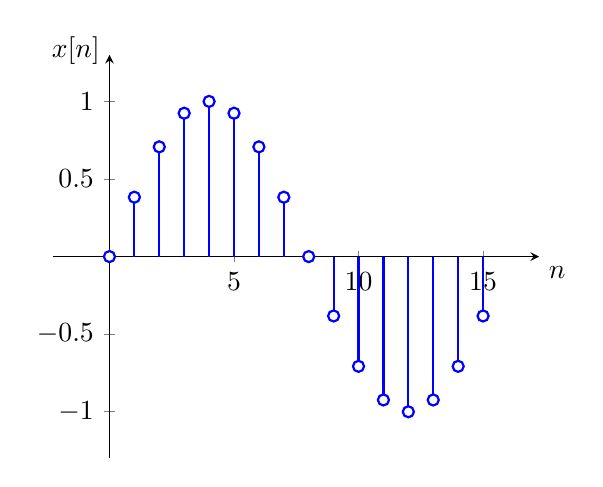
\begin{tikzpicture}
            \begin{axis}[%
                standard,
                scale=0.9,
                domain=0:15,
                samples=16,
                xlabel={$n$},
                ylabel={$x[n]$},
                ylabel style={yshift=10pt},
                ]
                \addplot+[ycomb,blue,thick] {sin(2*180*x/16)};
            \end{axis}
        \end{tikzpicture}
    \end{subfigure}
    \caption{Spojitý signál (vlevo) a~navzorkovaný signál (vpravo) vzorkovaný
    na frekvenci 16\,Hz}
    \label{pic:continuous-vs-sampled-signal}
\end{figure}

\subsection*{Kvantování}
\label{sub:quantization}

Pro převedení spojitého signálu na digitální nestačí pouze vzorkování.
Vzorkování diskretizuje časovou komponentu spojitého signálu na pevně daný
počet vzorků za jednotku času, ale nijak neovlivňuje hodnoty, kterých
jednotlivé vzorky mohou nabývat. Kvantování je proces diskretizace hodnot
zaokrouhlováním k~předem určeným hodnotám~\cite{Oliver1948}. Hodnoty nebo také
hladiny, ke kterým se zaokrouhluje, jsou dané počtem použitých bitů. Vyšší
počet bitů vede ke zlepšení kvality, protože zaokrouhlené hodnoty jsou blíže
jejich původním. Tento jev lze vidět na obrázku~\ref{pic:quantization}. Proces
kvantování vždy zavede do výsledného signálu takzvaný \textit{kvantizační šum}
\cite{Oliver1948}, protože převedení reálných čísel na digitální není exaktní.
Tento šum je rozdílem původního signálu a~kvantovaného signálu. Použití menšího
počtu bitů způsobí, že kvantizační šum bude výraznější, ale výsledný signál
bude mít menší velikost. Pro kvalitní audio se dnes nejčastěji používá alespoň
16~bitů.

\begin{figure}[hbt]
    \centering
    \begin{subfigure}[b]{0.5\linewidth}
        \centering
        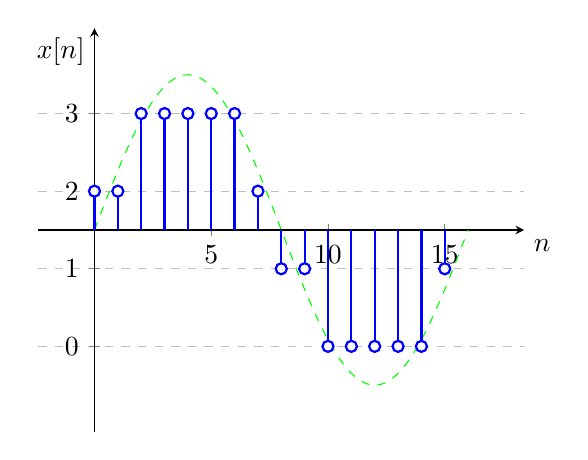
\begin{tikzpicture}
            \begin{axis}[%
                standard,
                scale=0.9,
                domain=0:16,
                xlabel={$n$},
                ylabel={$x[n]$},
                ytick={-1.5, -0.5, 0.5, 1.5},
                yticklabels={$0$, $1$, $2$, $3$},
                ymajorgrids=true,
                grid style=dashed,
                ]
                \addplot[green,dashed,samples=100] {2*sin(2*180*x/16)};
                \addplot+[ycomb,blue,thick,mark=*] coordinates{
                    (0,0.5)(1,0.5) (2,1.5) (3,1.5) (4,1.5) (5,1.5) (6,1.5)
                    (7,0.5) (8,-0.5) (9,-0.5) (10,-1.5) (11,-1.5) (12,-1.5)
                    (13,-1.5) (14,-1.5) (15,-0.5)
                };
            \end{axis}
        \end{tikzpicture}
    \end{subfigure}%
    \begin{subfigure}[b]{0.5\linewidth}
        \centering
        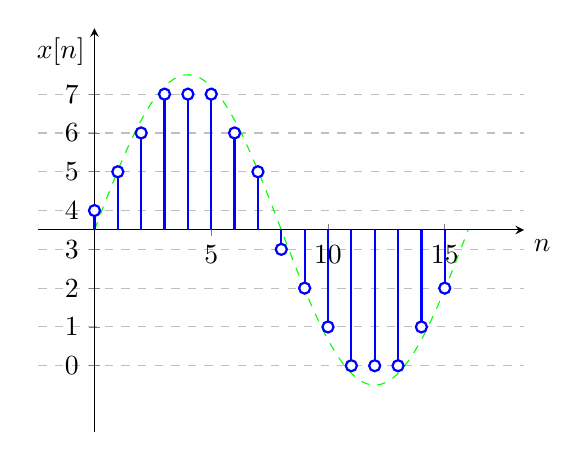
\begin{tikzpicture}
            \begin{axis}[%
                standard,
                scale=0.9,
                domain=0:16,
                xlabel={$n$},
                ylabel={$x[n]$},
                ytick={-3.5, -2.5, -1.5, -0.5, 0.5, 1.5, 2.5, 3.5},
                yticklabels={$0$, $1$, $2$, $3$, $4$, $5$, $6$, $7$},
                ymajorgrids=true,
                grid style=dashed,
                ]
                \addplot[green,dashed,samples=100] {4*sin(2*180*x/16)};
                \addplot+[ycomb,blue,thick,mark=*] coordinates{
                    (0,0.5)(1,1.5) (2,2.5) (3,3.5) (4,3.5) (5,3.5) (6,2.5)
                    (7,1.5) (8,-0.5) (9,-1.5) (10,-2.5) (11,-3.5) (12,-3.5)
                    (13,-3.5) (14,-2.5) (15,-1.5)
                };
            \end{axis}
        \end{tikzpicture}
    \end{subfigure}
    \caption{Signál z~obrázku~\ref{pic:continuous-vs-sampled-signal}
    vzorkovaný na frekvenci~16\,Hz a~kvantovaný na 2~bitech (vlevo) a~4~bitech
(vpravo)}
    \label{pic:quantization}
\end{figure}

Posledním krokem pro uložení a~přenos digitálních signálů je kódování vzorků.
Nejjednodušší způsob pro zakódování kvantovaných hodnot je převod na binární
čísla. Jednotlivé jedničky a~nuly pak mohou při přenosu reprezentovat
přítomnost pulzu~(1) a~nepřítomnost pulzu~(0). Tento systém, který obsahuje
vzorkování, kvantování a~kódování, se nazývá \textit{pulzně-kódová
modulace}~(PCM)~\cite{Oliver1948}. Pulzně-kódová modulace je důležitá obecně
pro zpracování digitálních signálů, ale i~pro účely této práce, protože ji
využívá zvukový formát \textit{Waveform Audio File Format}, který je popsán
v~následující podsekci.

\subsection*{Formáty digitálního zvuku}
\label{sub:digital-audio-formats}

Digitálních audio formátů je velké množství, každý se svými odlišnými
vlastnostmi. Hlavní kategorie, na které se digitální zvukové formáty dělí, jsou
\textit{nekomprimované} a~\textit{komprimované} -- ty se dále dělí na formáty
se ztrátovou a~bezeztrátovou kompresí. Příklady některých známých formátů jsou
v~tabulce~\ref{tab:audio-formats}.

\begin{table}[H]
    \vskip6pt
    \caption{Tabulka známých zvukových formátů}
    \vskip6pt
    \centering
    \begin{tabular}{lll}
        \toprule
        Nekomprimovaný & \multicolumn{2}{c}{Komprimovaný} \\
        \cmidrule(r){2-3}
                       & Bezeztrátový & Ztrátový \\
        \midrule
        WAV  & FLAC & MP3 \\
        AIFF & ALAC & AAC \\
        RAW  &      & OGG Vorbis \\
             &      & Opus \\
             &      & WebM \\
        \bottomrule
    \end{tabular}
    \label{tab:audio-formats}
\end{table}

Výhodou komprimovaných formátů je úspora datového prostoru. Naopak hlavní
nevýhodou komprimovaných formátů je složitější proces kódování a~dekódování. Se
vzorky komprimovaných formátů není možné přímo pracovat, ale je potřeba je
nejprve dekomprimovat a~převést do formátu, který umožňuje pracovat se
zvukovými daty přímo. Jedním z~nekomprimovaných formátů je \textit{Waveform
Audio File Format} (dále jen WAV). Jedná se o~proprietární formát pro digitální
audio vytvořený firmami Microsoft a~IBM. Je široce rozšířený a~není k~němu
potřeba žádná licence. Tento formát je nástavbou generického multimediálního
formátu \textit{Resource Interchange File Format} (RIFF). Konkrétní typ
pulzně-kódové modulace, který WAV formát nejčastěji používá je lineární
pulzně-kódová modulace (LPCM)~\cite{RFC2361} -- kvantovací úrovně mají mezi
sebou rovnoměrné rozestupy~\cite{LPCM}. Může ale používat i~jiné typy kódování,
jako \textit{IEEE Float} nebo komprimované \textmu-Law a~A-Law \cite{RFC2361}.

V~roce 2020 provedli AlSabhany, Ali, Ridzuan a~další~\cite{AlSabhany2020}
systematické srovnání 134~publikací zabývající se digitální zvukovou
steganografií a~zjistili, že 84\%~z~nich používalo formát WAV jako nosič. Za
účelem jednoduššího srovnávání metod bude tato práce pracovat pouze s~formátem
WAV.

\section{Digitální zvuková steganografie}
\label{sec:digital-audio-steganography}

Poslední dobou se začaly objevovat nové směry založené na steganografických
přístupech pro zajištění bezpečnosti a~utajení dat, které by v~kombinaci
s~konvenčními bezpečnostními technikami mohly vést k~lepším výsledkům
\cite{Djebbar2012}. Jedna z~konvenčních bezpečnostních technik kombinovaných se
steganografií je kryptografie. Zatímco steganografie se zabývá ukrýváním
informace, hlavním cílem kryptografie je převést zprávu do formy, která je pro
neoprávněné osoby nečitelná~\cite{AlSabhany2020}. I~když se tedy někdo pokusí
analyzovat komunikaci pro přítomnost utajené zprávy, není možné obsah rozeznat
od náhodného šumu.

Digitální zvuková steganografie má široké spektrum využití. Mezi praktické
příklady patří: monitorování reklam v~rádiu, indexování video nahrávek,
zachování soukromí jednotlivce, utajená komunikace mezi vojenskými rozvědkami
nebo bezpečnostními složkami a~použití všude tam, kde není možné použít
šifrování~\cite{Dutta2020}.

Dalším často používaným pojmem spojeným se steganografií je vodoznak. Vodoznaky
se používají pro vložení informací o~původu, vlastnictví, či autorských právech
dat~\cite{Djebbar2012}\cite{Dutta2020}\cite{Swanson1998}. Hlavní vlastností
vodoznaku je, že by nemělo být možné jej odstranit bez poškození nosného média.
Proto u~audia nesmí být součástí hlavičky souboru nebo být přenášen zvlášť, ale
být jeho součástí a~musí být nedetekovatelný. Musí být také odolný proti
transformaci signálu například při přenosu audia nebo převedení do formátu,
který používá ztrátovou kompresi~\cite{Swanson1998}. Velice známým příkladem
konvenčních vodoznaků jsou vodoznaky na bankovkách nebo \textit{žluté tečky}
v~tiskárnové steganografii -- známé také jako \textit{yellow dots} -- které
barevné tiskárny tisknou na každý list. Tyto tečky obsahují zakódované sériové
číslo tiskárny a~čas tisku~\cite{Dutta2020}. Pokud je vodoznak použit pro
ochranu intelektuálního vlastnictví, pak se ještě rozlišuje mezi vodoznakem
a~otiskem. Vodoznakem se značí všechny objekty stejně, ale otisk se může měnit
například pro každého zákazníka pro jeho pozdější identifikaci. To může být
užitečné, pokud poruší licenční podmínky například sdílením zakoupené
hudby~\cite{Swanson1998}.

\section{Vlastnosti a~jejich ověřování}
\label{sec:method-properties}

Aby bylo možné jednotlivé metody srovnávat mezi sebou, je nutné určit
vlastnosti, podle kterých budou hodnoceny. Těch může být mnoho, ale různí
autoři steganografických publikací se shodují, že nejvýznamnějšími vlastnostmi
jsou \textit{robustnost}, \textit{kapacita} a~\textit{nepostřehnutelnost}
\cite{AlSabhany2020}\cite{Djebbar2012}\cite{Dutta2020}. Tyto tři vlastnosti je
možné si představit jako trojúhelník s~každou vlastností v~jednom rohu, jak je
vidět na obrázku~\ref{pic:method-property-triangle}. Důvodem je fakt, že není
možné dosáhnout vysoké úrovně všech tří vlastností zároveň~\cite{Dutta2020}.
Zvýšení kvality jedné z~vlastností vždy vede ke snížení kvality alespoň jedné
zbývající~\cite{AlSabhany2020}\cite{Djebbar2012}. V~následujících podsekcích
budou popsány jednotlivé vlastnosti podrobněji. Bude také několikrát použit
pojem \textit{stego soubor}, což je soubor, který vznikne použitím určité
steganografické metody pro ukrytí zvolené informace do krycího souboru.

\begin{figure}[hbt]
    \centering
    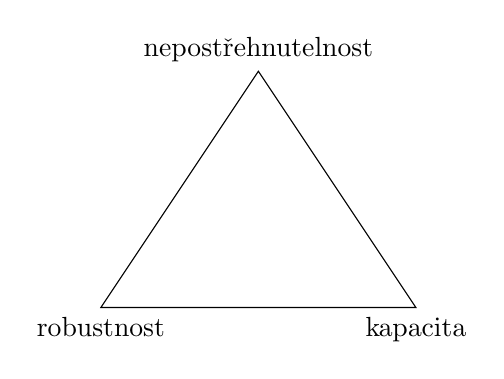
\begin{tikzpicture}
        \draw (0,0) coordinate[label=below:robustnost] --
              (4,0) coordinate[label=below:kapacita] --
              (2,3) coordinate[label=above:nepostřehnutelnost] --
              cycle;
    \end{tikzpicture}
    \caption{Trojúhelník se třemi nejvýznamnějšími vlastnostmi
    steganografických metod}
    \label{pic:method-property-triangle}
\end{figure}

\subsection*{Robustnost}
\label{sub:robustness}

Robustnost indikuje odolnost metody proti úmyslným či neúmyslným modifikacím
skrytých informací~\cite{AlSabhany2020}\cite{Dutta2020}. Míru robustnosti lze
hodnotit na základě množství skryté informace, která zůstane nezměněná po
různých úpravách stego souboru. Podle~\cite{Djebbar2012} mohou tyto modifikace
být:

\begin{itemize}
    \item zesílení amplitudy -- může poškodit skryté informace,
    \item filtrování -- skryté informace mohou být odstraněny filtrací určitého
        pásma,
    \item překvantování -- snížením počtu bitů a~zpětné překvantování na
        původní hodnotu zavede nejen kvantizační šum, ale může být poškozena
        nebo odstraněna skrytá informace,
    \item převzorkování -- podobná situace jako u~překvantování, snížení
        vzorkovací frekvence způsobí ztrátu informace,
    \item přidání šumu -- šum může skrytá data zamaskovat nebo poškodit,
    \item překódování -- skrytá informace může být poškozena převedením stego
        souboru do formátu, který používá ztrátovou kompresi.
\end{itemize}

Robustnost metody je obzvlášť důležitá pro tvorbu vodoznaku popsaného
v~podkapitole~\ref{sec:digital-audio-steganography}. Vodoznak musí být schopen
odolat výše zmíněným modifikacím, aby bylo možné správně identifikovat jeho
vlastníka~\cite{Swanson1998}.

\subsection*{Kapacita}
\label{sub:capacity}

Kapacita udává množství informace, které je možné do nosiče zakódovat a~úspěšně
dekódovat~\cite{Dutta2020}\cite{Djebbar2012}. Kapacitu metody je možné vyjádřit
v~bitech za sekundu ($bps$ nebo také $b/s$) nebo jako procentuální poměr
velikosti skryté informace k~velikosti nosiče
\cite{AlSabhany2020}\cite{Dutta2020}. Výhodou zvukových steganografických metod
je větší velikost souborů, se kterými metody pracují, což umožňuje ukrytí
většího množství informací. Zároveň je možné ukládat informace do nevyužitých
polí v~hlavičkách souborů \cite{Dutta2020}.

\subsection*{Nepostřehnutelnost}
\label{sub:imperceptibility}

Tato vlastnost vyjadřuje podobnost stego souboru a~krycího souboru a~je spojená
s~detekovatelností přítomnosti skryté informace~\cite{AlSabhany2020}. Úroveň
nepostřehnutelnosti je možné měřit pomocí \textit{perceptual evaluation of
speech quality} (PESQ) testu. Hodnota~4,5 znamená, že naměřený stego soubor je
totožný s~krycím souborem. Hodnota~1 indikuje maximální degradaci kvality.
Další způsob pro porovnání rozdílů dvou signálů je \textit{segmentový poměr
signálu k~šumu} (SegSNR)~\cite{Djebbar2012}. V~již zmíněné studii z~roku~2020
\cite{AlSabhany2020} zjistili autoři, že nejpoužívanější metodou napříč
analyzovanými publikacemi byl globální \textit{poměr signálu k~šumu} (SNR)
a~dále \textit{špičkový poměr signálu k~šumu} (PSNR).

Zvukové steganografické metody mají tu nevýhodu, že lidské zvukové ústrojí je
velmi citlivé, což ztěžuje ukrývání informací nepostřehnutelně. Přesto má
zvukové ústrojí nedostatky, které je možné využít, jako například maskování
tónu, který následuje po hlasitém impulzu. Dalším příkladem je maskování
informace, která je zakódovaná ve frekvenci zvuku, který se nachází
poblíž~\cite{Dutta2020}.

\section{Existující řešení}
\label{sec:existing-methods}

V~této podkapitole bude popsáno několik existujících metod digitální zvukové
steganografie. Popis každé metody bude obsahovat její princip a~silné a~slabé
stránky. Každý popis bude obsahovat konkrétní způsob jakým je možné zakódovat
a~dekódovat informace danou metodou. Na závěr každého popisu metody budou
diskutovány možnosti modifikace metody pro zlepšení některé ze
steganografických vlastností.

\subsection*{Metoda nahrazení nejméně významného bitu}
\label{sub:lsb}

Metoda využívající nahrazení nejméně významného bitu (anglicky \textit{least
significant bit substitution}, dále jen LSB) je nejjednodušší metodou pro
vkládání informací do nosiče. Principem této metody je nahrazení nejméně
významného bitu v~nosiči za bit ukrývané informace~\cite{Dutta2020}. Princip
kódování pomocí této metody je vizualizován na obrázku~\ref{pic:lsb-diagram}.

\begin{figure}[hbt]
    \centering
    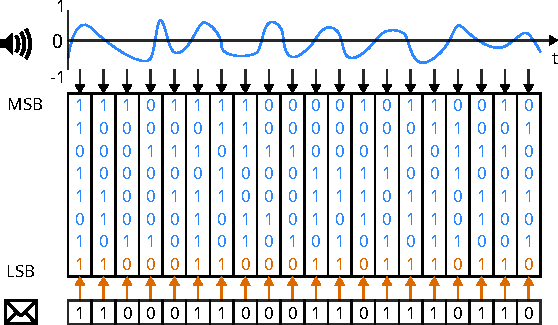
\includegraphics[width=0.8\textwidth]{obrazky/lsb-diagram.pdf}
    \caption{Ukládání informačních bitů do nejméně významného bitu krycího
    signálu. Upraveno z~\cite{Djebbar2012}.}
    \label{pic:lsb-diagram}
\end{figure}

Tato metoda se vyznačuje velmi vysokou kapacitou~\cite{Djebbar2012}
a~jednoduchou implementací. Kapacita této metody je přímo úměrná počtu a~bitové
hloubce vzorků nosiče. Je také vhodná pro kombinaci s~dalšími steganografickými
technikami~\cite{Djebbar2012}, jako je šifrování nebo komprese. Hlavní
nevýhodou této metody je její nízká robustnost. Informace ukryté LSB metodou je
velmi jednoduché poškodit triviálními úpravami stego souboru jako je například
zesílení, filtrace, přidání šumu, ztrátová komprese \cite{Djebbar2012},
převzorkování nebo překvantování. Robustnost této metody a~odolnost proti
některým z~těchto modifikací je možné zvýšit vkládáním do jiné bitové úrovně
než je poslední~\cite{Djebbar2012}.

Nemodifikovaná LSB metoda není příliš bezpečná, neboť je možné jednoduše vyčíst
hodnoty určité bitové úrovně a~tím odhalit ukryté informace~\cite{Djebbar2012}.
Pro lepší ukrytí informací je možné ukládat bity do náhodných vzorků
a~náhodných úrovní v~nich~\cite{Dutta2020}. Bezpečnost LSB metody je možné
zvýšit šifrováním ukrývaných informací. Ukrývaná data je vhodné nejprve
zkomprimovat například Lempel-Ziv-Welch (LZW) kompresí. Poté je možné je
zašifrovat vybraným šifrovacím algoritmem. Vhodným algoritmem pro symetrické
šifrování je \textit{Advanced Encryption Standard} (AES, česky standard
pokročilého šifrování). Pro asymetrické šifrování je vhodný algoritmus
Rivest-Shamir-Adleman (RSA)~\cite{Dutta2020}.

Kapacitu LSB metody je možné zvýšit například ukládáním do více bitových úrovní
za sebou v~jednotlivých vzorcích. Tato modifikace však produkuje šum, který je
lidské ucho schopno zachytit. Lepším způsobem, jak zvýšit kapacitu, je ukládání
do 4~nejnižších bitových úrovní pomocí algoritmu \textit{nahrazení nejmenší
chybou} (anglicky minimum-error replacement) a~rozprostření chyby do
následujících 4~vzorků. Tato modifikace zvyšuje kapacitu LSB metody o~33\%,
zatímco poměr signálu k~šumu je nižší než u~nemodifikované metody se stejným
počtem použitých bitů~\cite{Cvejic2002}.

\subsection*{Metoda skrývání pomocí ozvěny}
\label{sub:echo-hiding}

Steganografická metoda ukrývání informací pomocí ozvěny (anglicky \textit{echo
hiding}) funguje na principu přidání ozvěny do krycího
média~\cite{Djebbar2012}. Tato metoda má vyšší robustnost vůči filtrování,
převzorkování, či ztrátové kompresi. Lidské sluchové ústrojí má široký
dynamických rozsah výkonu a~frekvence, ale přesto je možné využít nedostatků,
jako je maskování tichých zvuků hlasitějšími~\cite{Gruhl1996}. Nevýhodou této
metody je zkreslení způsobené přidáním ozvěny do krycího média, které je
srovnatelné s~rozdílem poslechu audia ve sluchátkách a~přes reproduktory, kde
se zvuk odráží od stěn v~místnosti. Při vhodném nastavení parametrů je možné
docílit výborné nepostřehnutelnosti~\cite{Gruhl1996}. Těmito parametry jsou
indexy zpoždění, amplituda ozvěny a~míra exponenciálního dozvuku. Tato metoda
má dostatečnou míru robustnosti a~je tedy vhodná pro zakódování vodoznaku do
krycího média. Vhodné nastavení parametrů docílí velmi nízké pravděpodobnosti
odhalení či odstranění vodoznaku neoprávněnou osobou~\cite{Gruhl1996}. Po
přidání ozvěny si stego médium udrží stejné statistické a~percepční
vlastnosti~\cite{Djebbar2012}.

Pro implementaci této metody se krycí médium rozdělí na segmenty do kterých se
bity ukrývané informace zakódují vytvořením ozvěny daného segmentu. Pro
rozlišení hodnoty bitu se použije jiná míra zpoždění pro logickou~1
a~logickou~0. Kódování probíhá konvolucí segmentu a~konvolučním jádrem pro
příslušný bit. Jednotlivé segmenty se následně spojí a~přidají ke krycímu médiu
\cite{Gruhl1996}. V~praxi je ale výhodnější provést konvoluci krycího média
s~oběma konvolučními jádry a~použít bity ukrývané informace jako masku, která
určí jaké segmenty ponechat a~přidat ke krycímu médiu~\cite{Gruhl1996}. Pro
snížení míry zkreslení na rozmezí segmentů je vhodné vyhladit změnu mezi
hodnotou~0~a~1~\cite{Tekeli2017}. Příklad ozvěn, které vniknou použitím masky
bez vyhlazení přechodů mezi segmenty jsou na
obrázku~\ref{pic:echo-single-kernel-echo}. Příklad ozvěn, které vniknou
použitím masky s~vyhlazením přechodů jsou na obrázku
\ref{pic:echo-single-kernel-echo-smooth}.

\begin{figure}[hbt]
    \centering
    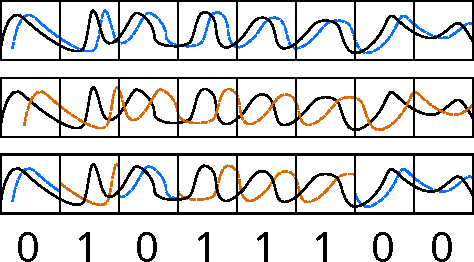
\includegraphics[width=0.8\textwidth]{obrazky/echo-diagram.pdf}
    \caption{Ozvěny vzniklé konvolucí s~konvolučními jádry pro jednu ozvěnu bez
    vyhlazení.}
    \label{pic:echo-single-kernel-echo}
\end{figure}

\begin{figure}[hbt]
    \centering
    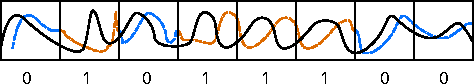
\includegraphics[width=0.8\textwidth]{obrazky/echo-smoothed.pdf}
    \caption{Ozvěny vzniklé konvolucí s~konvolučními jádry pro jednu ozvěnu
    s~vyhlazením přechodů mezi segmenty.}
    \label{pic:echo-single-kernel-echo-smooth}
\end{figure}

\subsubsection*{Ozvěna s~jedním konvolučním jádrem na bit}
\label{ssub:echo-single-kernel}

Tuto metodu poprvé představil Daniel Gruhl a~Walter Bender v~roce 1996
\cite{Gruhl1996}. Používá dvě konvoluční jádra dané rovnicí
\ref{eq:echo-single-kernel}, kde $\delta$ je Kroneckerova delta funkce, $d_i$
je zpoždění pro bit logické~0 a~logické~1 a~$\alpha$ je amplituda ozvěny
\cite{Dutta2020}.

\begin{equation}
    \label{eq:echo-single-kernel}
    h_i[n] = \delta[n] + \alpha\delta[n - d_i], i \in {0, 1}
\end{equation}

\noindent Zpožděné signály vniknou konvolucemi krycího média s~konvolučními
jádry dané rovnicí~\ref{eq:echo-single-kernel-echo}, kde $s[n]$ je krycí médium
a~$h_i[n]$ je konvoluční jádro z~rovnice~\ref{eq:echo-single-kernel}.

\begin{equation}
    \label{eq:echo-single-kernel-echo}
    k_i[n] = s[n] * h_i[n]
\end{equation}

\noindent Příklad ozvěn, které vniknou konvolucemi krycího média s~konvolučními
jádry jsou na obrázku~\ref{pic:echo-single-kernel-echo}.

\subsubsection*{Dekódování}
\label{ssub:echo-single-kernel-decoding}

K~dekódování této metody se používá cepstrální analýza. Stego signál se rozdělí
na stejný počet segmentů jako při kódování. Poté se vypočítá jejich cepstrum,
které je definováno jako inverzní Fourierova transformace ($\mathcal{F}^-1$)
logaritmu absolutní hodnoty Fourierovy transformace ($\mathcal{F}$) signálu
\cite{Tekeli2017}. Vzorec pro získání cepstra signálu $x(t)$ je definován
rovnicí~\ref{eq:cepstrum}.

\begin{equation}
    \label{eq:cepstrum}
    C = \mathcal{F}^-1(\log{|\mathcal{F}(x(t))|})
\end{equation}

\noindent Po výpočtu cepstra segmentu je možné zjistit hodnotu zakódovaného
bitu kontrolou, která hodnota na pozici $d_0$ a~$d_1$ je vyšší. Pokud je
hodnota $C(d_0)$ vyšší než $C(d_1)$, pak je hodnota bitu daného segmentu
logická~0. A~pokud je hodnota $C(d_1)$ vyšší než $C(d_0)$, pak je hodnota bitu
daného segmentu logická~1~\cite{Gruhl1996}. Příklad cepstra segmentu včetně
špiček na indexech zpoždění~100 a~110 lze vidět na
obrázku~\ref{pic:segment-cepstrum}.

\begin{figure}[hbt]
    \raggedright
    \begin{subfigure}[b]{0.4\linewidth}
        \centering
        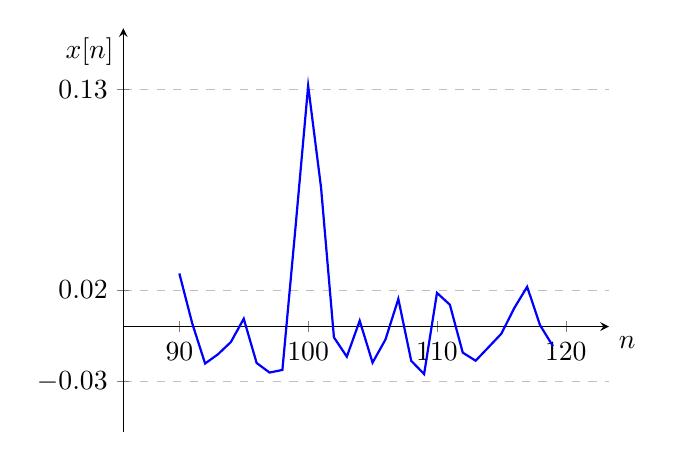
\begin{tikzpicture}
            \begin{axis}[%
                standard,
                enlarge y limits=0.2,
                scale=0.9,
                xlabel={$n$},
                ylabel={$x[n]$},
                scaled y ticks=false,
                y tick label style={/pgf/number format/fixed},
                ytick={-0.03, 0.02, 0.13},
                ymajorgrids=true,
                grid style=dashed,
                ]
                \addplot[blue,thick,samples=100] table [x={x}, y={y}] {
x y
90 0.02911713
91 0.00175175
92 -0.02027917
93 -0.01520897
94 -0.00849168
95 0.00427713
96 -0.01998557
97 -0.02522004
98 -0.02379227
99 0.05305905
100 0.13196956
101 0.07625496
102 -0.00591677
103 -0.01654206
104 0.00318564
105 -0.0197923
106 -0.00712777
107 0.01512758
108 -0.01878832
109 -0.0260548
110 0.01846125
111 0.01196165
112 -0.01430203
113 -0.01873781
114 -0.01135309
115 -0.00389159
116 0.01014747
117 0.02179004
118 0.00075464
119 -0.01072793
};
            \end{axis}
        \end{tikzpicture}
    \end{subfigure}\hspace{3em}%
    \begin{subfigure}[b]{0.4\linewidth}
        \centering
        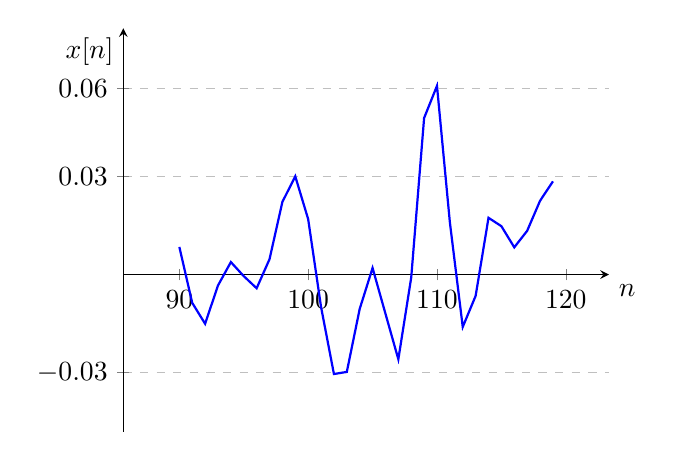
\begin{tikzpicture}
            \begin{axis}[%
                standard,
                enlarge y limits=0.2,
                scale=0.9,
                xlabel={$n$},
                ylabel={$x[n]$},
                scaled y ticks=false,
                y tick label style={/pgf/number format/fixed},
                ytick={-0.03, 0.03, 0.057},
                ymajorgrids=true,
                grid style=dashed,
                ]
                \addplot[blue,thick,samples=100] table [x={x}, y={y}] {
x y
90 0.00846854
91 -0.00866365
92 -0.01506901
93 -0.00334494
94 0.00382214
95 -0.00047939
96 -0.00419374
97 0.0046966
98 0.02226608
99 0.03008467
100 0.01698417
101 -0.00991495
102 -0.03046551
103 -0.02982553
104 -0.01053166
105 0.00202071
106 -0.01198137
107 -0.02595199
108 -0.00091994
109 0.04794415
110 0.05781149
111 0.01600666
112 -0.01603436
113 -0.00653139
114 0.01738747
115 0.014815
116 0.00833863
117 0.01340137
118 0.02259084
119 0.02855182
};
            \end{axis}
        \end{tikzpicture}
    \end{subfigure}
    \caption{Přiblížená cepstra segmentů. Levé kóduje logickou~0. Pravé kóduje
    logickou~1.}
    \label{pic:segment-cepstrum}
\end{figure}

Nevýhodou při dekódování této metody je například falešná detekce, pokud se ve
zvuku vyskytuje ozvěna, která nebyla vytvořena touto metodou. Dále může být
těžké detekovat informaci, pokud je amplituda ozvěny příliš malá a~špičky na
indexech zpoždění budou proto splývat s~okolím. Zesílení amplitudy zlepší míru
detekce, ale zvýší také náchylnost na neoprávněnou detekci~\cite{Kim2003}.

\subsubsection*{Modifikace metody skrývání pomocí ozvěny}
\label{ssub:echo-modifications}

Pro zvýšení robustnosti a~nepostřehnutelnosti použili autoři Oh, Seok, Hong
a~Youn~\cite{Oh2001} konvoluční jádro, které nejprve vytvoří ozvěnu se zápornou
a~poté s~kladnou amplitudou (anglicky bipolar echo). Zjistili, že tato
modifikace má vyšší míru robustnosti i~po překódování do ztrátového formátu
MP3. Dekódování této modifikace spočívá v~detekování špiček v~autokorelaci
výkonového cepstra. Výkonové cepstrum je podobné normálnímu cepstru a~je
definováno rovnicí~\ref{eq:power-cepstrum}.

\begin{equation}
    \label{eq:power-cepstrum}
    C_p = \mathcal{F}^-1(\log{|\mathcal{F}(x(t))|}^2)
\end{equation}

O~dva~roky později publikovali autoři Kim a~Choi~\cite{Kim2003} způsob, jak
znovu zvýšit robustnost pomocí konvolučního jádra se dvěma ozvěnami posunutými
vpřed i~vzad (anglicky backward-forward echo). Později publikovali autoři Wu
a~Chen \cite{Wu2006} modifikaci ozvěnové metody kombinující již popsané
modifikace. Ta používá konvoluční jádro pro vytvoření celkem čtyř ozvěn. Dvě
jsou posunuté vzad a~dvě vpřed přičemž obě strany mají ozvěnu s~kladnou
a~zápornou amplitudou. Autoři porovnávali tuto modifikaci s~výše popsanými
variantami této metody a~ve všech testech měla vyšší poměr úspěšně dekódovaných
bitů a~zároveň také vyšší poměr signálu k~šumu než ostatní varianty.

\subsection*{Metoda rozprostřeného spektra}
\label{sub:dsss}

Metoda rozprostřeného spektra byla nejprve vytvořena jako metoda pro zvýšení
spolehlivosti přenosu dat a~zajištění doručení informací. Ze stejných důvodů se
rozprostření spektra používá i~ve steganografii. Princip této metody spočívá
v~opakování informačních bitů $n$-krát podle čipové rychlosti (anglicky
\textit{chip rate}). Ta určuje, kolika bity bude kódován každý informační bit.
\cite{AlSabhany2020}. Dále popisované variantě této metody se říká přímé
rozprostřené spektrum (anglicky \textit{direct sequence spread spectrum}).

Kódování začíná převedením ukrývaných dat z~binárního formátu na čipy. Čip je
impulz, který používá hodnotu \textit{-1} místo binární hodnoty \textit{0}
a~hodnotu \textit{1} používá beze změny~\cite{Kuznetsov2022}. Poté je každý bit
vynásoben pseudonáhodnou čipovou sekvencí $n$-krát, čímž dojde k~rozprostření
informačních bitů přes více přenesených bitů. Zvýšení počtu kopií bitů zvýší
robustnost a~zároveň sníží kapacitu této metody~\cite{AlSabhany2020}. Výsledné
stego médium vznikne přidáním vynásobených hodnot ke krycímu médiu
\cite{Kuznetsov2022}. Informace zakódovaná touto metodou je odolná proti šumu,
protože obsahuje přebytečné kopie bitů. V~případě poškození části stego média
je možné z~přebytečných bitů obnovit ukryté informace~\cite{Djebbar2012}.
Popsaný princip kódování je možné vidět na obrázku~\ref{pic:dsss-spreading},
kde se ke krycímu signálu přidají rozprostřené bity informace vynásobené
pseudonáhodnou sekvencí čipů.

\begin{figure}[hbt]
    \centering
    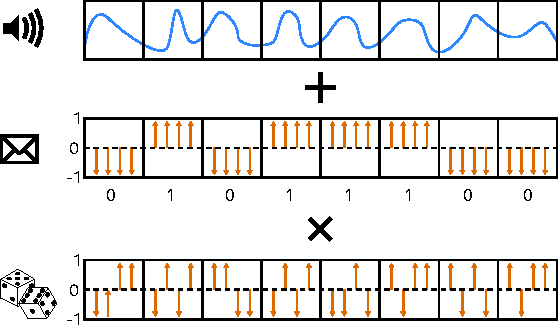
\includegraphics[width=0.8\textwidth]{obrazky/direct-sequence-spread-spectrum-diagram.pdf}
    \caption{Kódování rozprostřených bitů (uprostřed) pomocí metody přímého
    rozprostření spektra vynásobením s~pseudonáhodnou sekvencí (dole)
    a~přidáním ke krycímu signálu (nahoře).}
    \label{pic:dsss-spreading}
\end{figure}

Tato metoda je dostatečně robustní pro přidání více vodoznaků. Například pro
přidání více autorů k~hudební skladbě. Při detekci konkrétního vodoznaku jsou
ostatní považovány jako šum. Dále je tato metoda dostatečně robustní vůči
přidanému šumu a~překódování do ztrátového formátu~\cite{Boney1996}. Aby byl
náhodný šum přidaný touto metodou neslyšitelný, je nutné nastavit při kódování
amplitudu rozprostřené sekvence zhruba na 0,5\% dynamického rozsahu krycího
média~\cite{Bender1996}. Pro kvalitní dekódování má tato metoda kapacitu 4~bity
za sekundu~\cite{Bender1996}.

Pro dekódování informačních bitů je nezbytné, aby příjemce měl stejnou
pseudonáhodnou sekvenci čipů, která byla použita k~zakódování. Pro dekódování
se stego médium a~pseudonáhodná sekvence rozdělí na segmenty a~vypočítá se
korelace mezi každým segmentem stego média a~pseudonáhodné sekvence. Pro určení
hodnoty bitu je možné použít rozhodovací pravidlo v~rovnici
\ref{eq:dsss-decision-rule}, kde $b$ je hodnota bitu a~$c$ je výsledek
korelace~\cite{Kuznetsov2022}.

\begin{equation}
    \label{eq:dsss-decision-rule}
    b = \left\{
        \begin{array}{rl}
            0, & c < 0 \\
            1, & c > 0
        \end{array}
    \right.
\end{equation}

\subsection*{Metoda fázového kódování}
\label{sub:phase-coding}

Metoda fázového kódování je založená na nahrazení fáze prvního segmentu audia
referenční fází reprezentující ukrývaná data. Fáze následujících segmentů je
upravena tak, aby byla zachována relativní fáze mezi segmenty. Metoda fázového
kódování dosahuje nejlepších hodnot poměru signálu k~šumu. Avšak příliš velká
změna fáze frekvenční komponenty vede k~rozptylu fáze a~tím ke zhoršení kvality
zvuku. Dokud jsou ale změny fáze dostatečně malé, což je subjektivní, pak je
možné dosáhnout neslyšitelného kódování~\cite{Bender1996}.

Kódování pomocí této metody začíná rozdělením krycího audia na segmenty
s~délkou počtu ukrývaných bitů. Poté je každý segment převeden do frekvenční
domény pomocí Fourierovy transformace. Z~transformovaného signálu je možné
vytvořit matici fází -- značeno $\phi_n(\omega_k)$ -- a~matici amplitud
segmentů -- značeno $A_n(\omega_k)$. Písmeno $n$ značí index segmentu a~písmeno
$k$ značí index vzorku uvnitř segmentu. Poté se vypočítá rozdíl fází segmentů
napříč řádky~\cite{Bender1996}. Matematický zápis rozdílu fází je v~rovnici
\ref{eq:phase-diff}.

\begin{equation}
    \label{eq:phase-diff}
    \Delta\phi_n(\omega_k) = \phi_{n+1}(\omega_k) - \phi_n(\omega_k)
\end{equation}

\noindent Poté se bity ukrývaných dat převedou do formátu $\frac{\pi}{2}$
reprezentující hodnotu~0 a~$-\frac{\pi}{2}$ reprezentující hodnotu~1. Touto
sekvencí se nahradí první segment v~matici fází. Poté se postupně počítají nové
fáze z~původní fázové matice a~matice rozdílů fází. Matematický zápis je
v~rovnici~\ref{eq:new-phases}, kde $\phi'$ značí novou matici fází a~$N$
značí index posledního segmentu~\cite{Bender1996}.

\begin{equation}
    \label{eq:new-phases}
    \left[
        \begin{array}{lclcl}
            \phi_1'(\omega_k) & = & \phi_0'(\omega_k)     & + & \Delta\phi_1(\omega_k) \\
            \phi_n'(\omega_k) & = & \phi_{n-1}'(\omega_k) & + & \Delta\phi_n(\omega_k) \\
                              & \vdots \\
            \phi_N'(\omega_k) & = & \phi_{N-1}'(\omega_k) & + & \Delta\phi_N(\omega_k)
        \end{array}
    \right]
\end{equation}

\noindent Na závěr je možné sestavit stego signál z~amplitud a~nových fází
pomocí inverzní Fourierovy transformace~\cite{Bender1996}. Z~obou matic je
potřeba zkombinovat hodnoty amplitud a~fází v~jednotlivých segmentech pro
vytvoření komplexních čísel v~exponenciálním tvaru. Na každý segment se poté
aplikuje inverzní Fourierova transformace. Tyto segmenty se znovu spojí
dohromady, čímž vznikne výsledné stego médium. Dekódování probíhá pouhým
převedením fází z~prvního segmentu stego média na bity stejným způsobem jako
při kódování.

Kapacita této metody se pohybuje v~rozsahu 8~bitů za sekundu až 32~bitů za
sekundu podle množství šumu přítomného v~krycím médiu. Více šumu vede k~vyšší
kapacitě~\cite{Bender1996}. Existují modifikace této metody, které využívají
jiné fáze krycího signálu. Například vyšší frekvence jsou hůře detekovatelné
lidským sluchovým ústrojím~\cite{Djebbar2014}. Autoři~\cite{Djebbar2014}
vybírají pro kódování pouze frekvenční regiony s~vysokou energií.

\subsection*{Metoda paritního kódování}
\label{sub:parity-coding}

Metoda paritního kódování je založená na ukrývání do nejméně významného bitu
skupiny vzorků na rozdíl od ukrývání do jednotlivých vzorků. Pro zakódování
informace se krycí médium rozdělí na segmenty a~vypočítá se paritní bit
segmentu. Pokud je paritní bit stejný jako informační, pak se neprovádí nic.
Pokud je paritní bit rozdílný, pak se změní nejméně významný bit libovolného
vzorku v~daném segmentu. Díky tomu je možné snížit detekovatelnost informace
\cite{Bandyopadhyay2008}, čímž ale dojde ke snížení robustnosti. Způsob
kódování pomocí této metody je vizualizován na obrázku~\ref{pic:parity-coding}.

\begin{figure}[hbt]
    \centering
    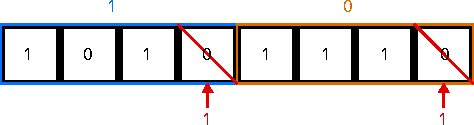
\includegraphics[width=0.8\textwidth]{obrazky/parity-coding.pdf}
    \caption{Metoda paritního kódování. Pro zakódování je potřeba docílit
    stejné parity jako je informační bit.}
    \label{pic:parity-coding}
\end{figure}

\subsection*{Metody založené na nedostatcích lidského sluchového ústrojí}
\label{sub:has}

Tyto metody byly využívány již od počátků steganografie a~využívají percepčních
vlastností lidského sluchového ústrojí a~psychoakustických vlastností řeči.
Tyto metody využívají maskování v~časové nebo frekvenční doméně. Maskování
v~časové doméně využívá nutnosti počkat chvíli po zaslechnutí hlasitého tónu.
Pro ukrytí určitého tónu je možné vložit jej do bezprostřední blízkosti
hlasitého impulzu. Nápodobně, maskování ve frekvenční doméně probíhá vložením
frekvence, která se nachází v~blízkém okolí jiné frekvence s~vyšší
amplitudou~\cite{Dutta2020}.

Jedna z~metod pracující ve frekvenční doméně je metoda vkládání tónu
\cite{Dutta2020}. Ta spoléhá na neschopnost vnímání tónu v~přítomnosti mnohem
hlasitějších. Pro kódování se krycí médium rozdělí na segmenty a~vypočítá se
výkon každého z~nich. Poté se vloží dva tóny na frekvencích $f_0$ a~$f_1$.
Výkony tónů jsou nastaveny v~předem známém poměru k~výkonu segmentu
\cite{Djebbar2012}. Princip kódování této metody lze vidět na obrázku
\ref{pic:tone-insertion}, kde poměr výkonů tónu na frekvencích $f_0$ a~$f_1$
kóduje bity \texttt{010}.

\begin{figure}[hbt]
    \centering
    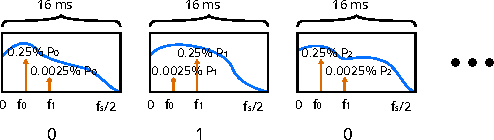
\includegraphics[width=\textwidth]{obrazky/tone-insertion-diagram.pdf}
    \caption{Metoda vkládání tónu. Specifické poměry tónů na frekvencích $f_0$
    a~$f_1$ kódují 0~nebo~1.}
    \label{pic:tone-insertion}
\end{figure}

Dekódování probíhá porovnáním poměrů výkonu segmentu k~výkonu tónu na dané
frekvenci~\cite{Djebbar2012}. Dekódovací pravidlo lze vidět v~rovnici
\ref{eq:tone-insertion-decision-rule}, kde $b$ značí hodnotu bitu a~výkon
segmentu je označen jako $P_i$, přičemž $i$ značí index segmentu a~$f_0$~a$f_1$
značí použité frekvence.

\begin{equation}
    \label{eq:tone-insertion-decision-rule}
    b = \left\{
        \begin{array}{rl}
            0, & \frac{P_i}{P_{f_0}} > \frac{P_i}{P_{f_1}} \\
            1, & \mathrm{jinak}
        \end{array}
    \right.
\end{equation}

\noindent Tato metoda má malou kapacitu a~vložené tóny je jednoduché detekovat,
proto je vhodné použít čtyři a~více párů frekvencí, které se střídají na
základě určitého klíče~\cite{Djebbar2012}.

\subsection*{Metoda ukrývání v~úsecích ticha}
\label{sub:hiding-in-silence-intervals}

Tato metoda využívá ke skrývání informací úseky ticha nacházející se
v~nahrávkách řeči~\cite{Djebbar2012}. Pro zakódování informací je nejprve
potřeba najít úseky ticha v~nahrávce. Ty se vyskytují jako posloupné sekvence
vzorků s~amplitudou nižší než určitá hodnota. Z~nalezených úseků se ponechají
pouze ty, jejichž délka je větší než minimální délka úseku~\cite{Shahreza2008}.
Autoři~\cite{Shahreza2008} zjistili následující optimální hodnoty:

\begin{itemize}
    \item maximální amplituda úseku: 15\% maximálního rozsahu signálu,
    \item minimální délka úseku: 200~vzorků; kratší úseky se většinou vyskytují
        mezi částmi slov a~tyto skoky mohou být detekovány,
    \item maximální počet bitů pro ukrytí do segmentu: 4~b.
\end{itemize}

\noindent Pokud $X$ je kódovaná hodnota, $N$ je počet bitů kódované hodnoty
a~$L$ je délka konkrétního segmentu, pak pro kódování do konkrétního segmentu
se vypočítá jeho nová délka $D$, tak aby platil vztah v~rovnici
\ref{eq:silence-value}~\cite{Shahreza2008}.

\begin{equation}
    \label{eq:silence-value}
    X = D \bmod 2^N
\end{equation}

\noindent Novou délku segmentu lze jednoduše vypočítat z~rovnice
\ref{eq:silence-length}.

\begin{equation}
    \label{eq:silence-length}
    D = L - [(L - X) \bmod 2^N]
\end{equation}

\noindent Pokud by byla nová délka $D$ kratší než je minimální stanovená délka
úseku, pak je potřeba použít jiný úsek. Pro dekódování informace stačí použít
zmíněný vztah~\ref{eq:silence-value}~\cite{Shahreza2008}.

Nevýhodou této metody je její citlivost na transformaci stego signálu. Změny
délek úseků ticha povedou k~dekódování špatných hodnot. Pro zvýšení robustnosti
v~tomto ohledu je možné snížit amplitudu úseků ticha a~zvýšit amplitudu
okolních úseků, aby nedošlo ke změně délky některého z~úseků například kvůli
kompresi~\cite{Djebbar2012}.

\subsection*{Metoda využívající vlnkové transformace}
\label{sub:wavelet-transform}

Nejlepší metodou pro ukrývání informací v~transformační doméně je diskrétní
vlnková transformace (anglicky \textit{discrete wavelet transform}, dále jen
DWT), protože prezentuje informace o~frekvencích, které lze získat z~Fourierovy
transformace jako funkci v~čase. Vlnková transformace poskytuje dobrý kompromis
mezi časovou doménou signálu a~frekvenční doménou, protože Fourierova
transformace frekvencím nepřiřazuje čas. Další transformační funkcí je
diskrétní kosinová transformace (anglicky \textit{discrete cosine transform} --
DCT). Ta není pro účely ukrývání informací příliš vhodná, protože zavádí do
audia artefakty. Metody v~transformační doméně jsou poměrně méně odolné proti
šumu~\cite{Dutta2020}.

Pro zakódování informace do nosiče pomocí DWT se nosič rozdělí na segmenty po
512~vzorcích. Na každý segment je pětkrát aplikována dekompozice na
nízkofrekvenční a~vysokofrekvenční komponenty~\cite{Cvejic2002Wavelet}. Každá
následující dekompozice je aplikována na nízkofrekvenční složku z~předchozí
úrovně~\cite{Prabakaran2012}. Výsledných 512~koeficientů je převedeno na
binární hodnoty do jejichž nejméně významných bitů jsou uloženy bity ukrývané
informace~\cite{Cvejic2002Wavelet}. Experimentální výsledky
v~\cite{Cvejic2002Wavelet} ukázaly, že při modifikaci až 7~nejnižších bitů bylo
téměř nemožné rozeznat rozdíl mezi originální a~upravenou nahrávkou. A~i~při
modifikaci více úrovní byly výsledky lepší než při použití konvenční metody
nahrazení nejméně významného bitu popsané v~podsekci~\ref{sub:lsb} s~dvakrát
menším počtem upravených bitových úrovní. Tato metoda má velmi vysokou kapacitu
a~je schopna ukrýt až o~220,5\,kb/s více dat než konvenční metoda nahrazení
nejméně významného bitu~\cite{Cvejic2002Wavelet}.

Proces dekódování probíhá podobně jako kódování. Stego signál se rozdělí na
segmenty, provede se dekompozice a~koeficienty se převedou na binární hodnoty.
Z~nejnižších bitů je možné vyčíst bity ukryté informace~\cite{Pooyan2007}.


\chapter{Analýza a~návrh}
\label{cha:library-design}

V~této kapitole bude popsán řešený problém a~konceptuální návrh řešení. Bude
popsána struktura softwarové knihovny a~vestavěného programu pro zvukovou
steganografii a~vysokoúrovňový popis struktury projektu, použitých technik
a~metod k~tvorbě kvalitního a~rozšiřitelného řešení. Budou také popsány použité
softwarové nástroje a~na závěr kapitoly bude popsán princip navrhované metody
pro digitální zvukovou steganografii.

\section{Rozbor řešeného problému}
\label{sec:problem-analysis}

Hlavním problémem v~tomto oboru je nedostatek kvalitně implementovaných řešení,
přestože je množství literatury poměrně bohaté. Velké množství existujících
řešení je zastaralých a~často nepodporují volbu steganografické metody.

% \subsection*{Požadavky řešení}
% \label{sub:solution-requirements}

% \todo{pozadavky reseni}
% \blindtext

% \subsection*{Metody a~prostředky řešení problému}
% \label{sub:problem-solution}

% \todo{prostředky řešení problému}
% \blindtext

\subsection*{Výhody a~nevýhody stávajících řešení}
\label{sub:pros-cons-existing-solutions}

V~celém oboru steganografie je těžké najít kvalitní existující řešení. Většina
existujících řešení má dva společné problémy: málo implementovaných metod
a~špatnou dokumentaci. Zde je seznam nalezených řešení a~krátký popis každého
z~nich:

\begin{itemize}
    \item \textit{Steghide}\footnote{\url{https://steghide.sourceforge.net}} --
        Jedno z~lepších nalezených řešení. Jedná se o~svobodný software s~GPL
        licencí, podporuje šifrování pomocí algoritmu \textit{AES-128}
        a~používá grafový algoritmus pro kódování. Program je ale velmi
        zastaralý a~nepodporuje jiné metody kódování.
    \item \textit{Hide4PGP}\footnote{\url{http://www.heinz-repp.onlinehome.de/Hide4PGP.htm}}
        -- Další otevřený software s~podporou šifrování pomocí
        \textit{OpenPGP}\footnote{\url{https://www.openpgp.org}}. Kódování
        rozprostírá informační bity přes celý soubor.
    \item \textit{Xiao Steganography}\footnote{\url{https://download.cnet.com/Xiao-Steganography/3000-2092_4-10541494.html}}
        -- Proprietární program s~podporou pěti šifrovacích a~čtyř hešovacích
        algoritmů, které jsou avšak velmi zastaralé a~jejich používání se
        nedoporučuje.
    \item \textit{audio-steganography-algorithms}\footnote{\url{https://github.com/ktekeli/audio-steganography-algorithms}}
        -- Sada implementací metod pro program MATLAB. Obsahuje metodu
        rozprostřeného spektra (viz podsekce~\ref{sub:dsss}), ukrývání pomocí
        ozvěny (viz podsekce~\ref{sub:echo-hiding}), nejméně významného bitu
        (viz podsekce~\ref{sub:lsb}) a~fázového kódování (viz
        podsekce~\ref{sub:phase-coding}). Bohužel jsou modifikace metod
        v~nečitelném proprietárním formátu.
    \item \textit{Steganography}\footnote{\url{https://github.com/ragibson/Steganography}}
        -- Program v~jazyce \textit{Python}. Pro audio soubory ve formátu
        \textit{WAV} podporuje pouze metodu nahrazení nejméně významného bitu.
    \item \textit{Audio steganography - Phase encoding}\footnote{\url{https://github.com/dan-oak/secret_in_wav}}
        -- Ukázkový program v~jazyce Python pro kódování pomocí metody fázového
        kódování.
    \item \textit{py-stego-phase}\footnote{\url{https://github.com/Galarius/py-stego-phase}}
        -- Další program v~jazyce Python pro metodu fázového kódování.
    \item \textit{InvisibleSecrets}\footnote{\url{https://www.east-tec.com/invisiblesecrets}}
        -- Proprietární program s~podporou šifrování.
    \item \textit{StegoStick}\footnote{\url{https://sourceforge.net/projects/stegostick}}
        -- Svobodný software s~podporou šifrování, avšak zastaralého.
    \item \textit{DeepSound}\footnote{\url{https://jpinsoft.net/DeepSound/Overview.aspx}}
        -- Proprietární program s~podporou šifrování. Šifrovací algoritmus je
        současně nejvíce doporučovaný algoritmus \textit{AES-256}.
\end{itemize}

\section{Návrh řešení}
\label{sec:solution-proposal}

Řešením problému je vytvoření softwarové knihovny a~programu, která bude
implementovat steganografické metody popsané v~sekci
\ref{sec:existing-methods}. Aby bylo řešení jednoduše rozšiřitelné, bude použit
objektově orientovaný návrh. Každá ze steganografických metod bude mít společné
rozhraní, aby bylo použití a~implementace nových metod co nejjednodušší. Dalším
požadavkem na řešení je, aby bylo čitelné a~jednoduše pochopitelné. Musí zde
být však určitý kompromis mezi čitelností a~optimalizací kódu. Řešení by mělo
být relativně rychlé a~proto by kódování mělo probíhat v~řádech několika sekund
až minut.

Při volbě tajné zprávy bude mít uživatel programu na výběr textový vstup nebo
obsah souboru. Rozhraní jednotlivých metod bude pracovat s~bity ukrývané
informace, díky čemuž nebude záležet na typu kódovaných dat. Pro kódování je
tedy postačí převést z~bajtů na bity a~při dekódování naopak. Většina
steganografických metod má několik parametrů které mají vliv na robustnost,
kapacitu a~nepostřehnutelnost metody. Tyto parametry budou uživateli
zpřístupněny jako dodatečné argumenty při spouštění programu nebo při kódování
a~dekódování v~knihovní části této práce.

Z~metod popsaných v~sekci~\ref{sec:existing-methods} jsem plánoval
implementovat všechny, avšak některé metody se ukázaly být velmi složité na
implementaci. Implementována nebude metoda vlnkové transformace a~také metoda
paritního kódování, protože se jedná prakticky o~modifikaci metody nahrazení
nejméně významného bitu. U~metod vybraných k~implementaci budou také
implementovány některé popsané modifikace metod.

\subsection*{Blokové schéma a~komponenty systému}
\label{sub:solution-components}

Struktura řešení se bude skládat z~několika modulů a~balíčků. Pro zjednodušení,
modul je jeden soubor a~balíček je kolekce modulů. Jádrem knihovny bude balíček
s~moduly implementovaných metod pro digitální zvukovou steganografii. Druhý
hlavní balíček bude obsahovat moduly týkající se vestavěného programu
s~terminálovým rozhraním. Nejdůležitějším modulem pro programovou část bude
modul s~fasádou, která zjednoduší volání jednotlivých metod při použití
z~terminálu. Bude také poskytovat výpočty různých statistických funkcí na
základě kterých bude možné vyhodnotit pro konkrétní krycí soubor úroveň
jednotlivých vlastností steganografických metod popsaných v~sekci
\ref{sec:method-properties}. Blokové schéma popsané struktury je možné vidět na
obrázku~\ref{pic:library-block-diagram}.

\begin{figure}[hbt]
    \centering
    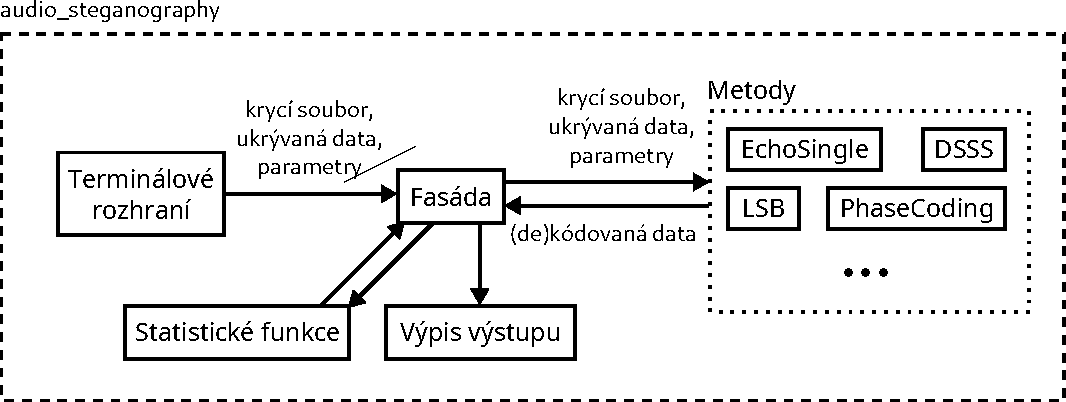
\includegraphics[width=\textwidth]{obrazky/block-diagram.pdf}
    \caption{Blokové schéma knihovny pro digitální zvukovou steganografii}
    \label{pic:library-block-diagram}
\end{figure}

\subsection*{Realizační prostředky a~metody}
\label{sub:solution-tool-choices}

K~implementaci navrženého řešení jsem zvolil programovací jazyk \textit{Python}
minimální verze~\textit{3.8}. Tento jazyk jsem vybral, protože je to
vysokoúrovňový jazyk s~dobře čitelnou syntaxí. Je také dynamicky typovaný
a~umožňuje kombinovat objektově orientovaný a~funkcionální styl programování,
díky čemu je možné psát elegantní kód. Další kvalitou je dobré rozhraní
s~jazykem~\textit{C}, díky kterému mohou být knihovny velmi rychlé. Jednou
takovou knihovnou je knihovna \textit{NumPy}\footnote{\url{https://numpy.org}},
která poskytuje optimalizované funkce pracující s~vícedimenzionálním polem
jménem \textit{NDArray}. Na této datové struktuře a~funkcích staví celá řada
dalších numerických knihoven, jako například knihovna
\textit{SciPy}\footnote{\url{https://scipy.org}}, která pomocí NumPy
implementuje velké množství funkcí pro účely zpracování signálů. Další
knihovnou, která využívá NumPy je knihovna
\textit{pandas}\footnote{\url{https://pandas.pydata.org}}, která slouží pro
zpracování dat. Tato knihovna bude použita pro zpracování dat vygenerovaných
při vyhodnocování vlastností metod.

Kód bude strukturován podobně jako jiné knihovny a~balíčky pro jazyk Python.
Obecně obsahují Python knihovny primárně: zdrojový kód, konfigurační soubory
pro vytvoření balíčku k~distribuci, softwarovou licenci a~soubor
\texttt{README.md}, který obsahuje případné prerekvizity a~příklady použití či
spuštění. Jako softwarovou licenci pro tento projekt jsem zvolil licenci
\textit{Apache-2.0}, protože je velmi otevřená -- dovoluje i~komerční použití
a~distribuci bez zdrojového kódu -- a~je také často používaná Python
knihovnami.

\subsection*{Případy užití}
\label{sub:use-cases}

Program bude umožňovat uživateli zvolit steganografickou metodu a~pomocí ní
zakódovat a~dekódovat tajnou zprávu ve formě textu nebo souboru do krycího
audio souboru. Interakci mezi použitím hlavního programu a~knihovny je možné
vidět na obrázku~\ref{pic:use-case-diagram-main}.

\begin{figure}[hbt]
    \centering
    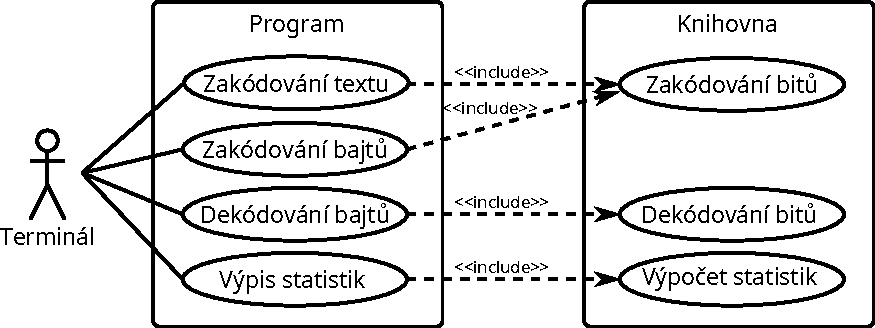
\includegraphics[width=\textwidth]{obrazky/use-case-diagram-1.pdf}
    \caption{Diagram případů užití primárního vestavěného programu a~knihovny.}
    \label{pic:use-case-diagram-main}
\end{figure}

Druhý vestavěný program bude umožňovat testování jednotlivých steganografických
vlastností. Diagram případů užití pro druhý program je na obrázku
\ref{pic:use-case-diagram-testing}.

\begin{figure}[hbt]
    \centering
    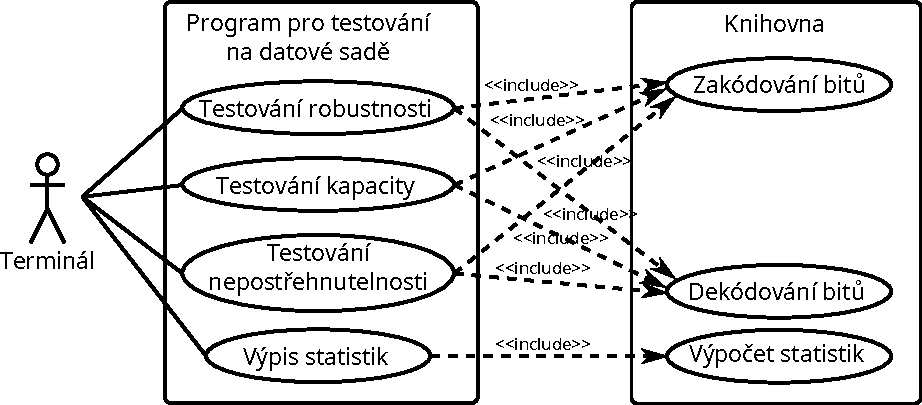
\includegraphics[width=\textwidth]{obrazky/use-case-diagram-2.pdf}
    \caption{Diagram případů užití druhého vestavěného programu pro testování
    steganografických vlastností na datové sadě.}
    \label{pic:use-case-diagram-testing}
\end{figure}

\subsection*{Ověřování vlastností}
\label{sub:method-property-verification}

Pro ověření vlastností steganografických metod bude součástí knihovny druhý
vestavěný program, který bude systematicky testovat jednotlivé vlastnosti každé
metody. Testování bude probíhat na často používaných datových sadách pro
digitální zvukovou steganografii. Podle~\cite{AlSabhany2020} jsou to tyto
datové sady: \textit{GTZAN} \cite{Tzanetakis2001},
\textit{Noizeus}~\cite{Hu2006} a~\textit{UrbanSound8K} \cite{Salamon2014}.
K~těmto datovým sadám jsem ještě přidal vlastní sadu souborů, která bude
s~ostatními více popsána níže.
Podle~\cite{AlSabhany2020} patří mezi používané sady také datový korpus
\textit{TIMIT}~\cite{Garofolo1993}, avšak ten zde nebude testován.

Hodnoty jednotlivých vlastností se vyčíslují pomocí statistických funkcí, které
se často objevovaly v~průzkumu~\cite{AlSabhany2020}. Tyto funkce jsou:

\begin{itemize}
    \item poměr signálu k~šumu měřen v~decibelech (anglicky
        \textit{signal-to-noise ratio}, dále jen SNR),
    \item špičkový poměr signálu k~šumu měřen v~decibelech (anglicky
        \textit{peak signal-to-noise ratio}, dále jen PSNR),
    \item míra bitové chybovosti (anglicky \textit{bit error rate}, dále jen
        BER),
    \item střední kvadratická chyba (anglicky \textit{mean squared error}, dále
        jen MSE),
    \item směrodatná odchylka (anglicky \textit{root-mean-square deviation},
        dále jen RMSD).
\end{itemize}

\noindent Rovnice těchto funkcí jsou v~příloze~\ref{cha:statistical-functions}.
Při testování se nejprve vyhodnotí maximální kapacita metody bez modifikace
stego signálu s~pomocí funkce BER. Poté bude testována robustnost následujícími
metodami zvlášť i~kombinovaně:

\begin{itemize}
    \item přidání šumu,
    \item filtrace spektra,
    \item převzorkování,
    \item překvantování,
    \item překódování do ztrátového formátu.
\end{itemize}

\noindent Nepostřehnutelnost je sice subjektivní vlastnost, ale je možné
částečně vyhodnotit její míru automaticky pomocí úrovně SNR a~PSNR.

\subsubsection{Popis použitých datových sad}
\label{ssub:dataset-descriptions}

Datová sada \textit{GTZAN} vznikla mezi lety 2000-2001 a~obsahuje
1000~hudebních nahrávek po 30~sekundách. Žánr a~zdroj jednotlivých nahrávek je
různorodý. Datová sada obsahuje celkem 10~hudeních žánrů. Nahrávky obsahují
jeden kanál a~jsou vzorkovány na frekvenci 22050\,Hz a~kvantovány na
16~bitech~\cite{Tzanetakis2001}.

Datová sada \textit{NOIZEUS} vnikla v~roce~2007 za účelem lepšího srovnání
algoritmů pro zkvalitnění hlasových dat. Sada obsahuje 30~nahrávek s~jedním PCM
kanálem vzorkovaným na frekvenci 8\,kHz a~kvantovaným na 16~bitech. Obsahem
nahrávek jsou všechny fonémy americké angličtiny. Součástí sady je také osm
modifikovaných verzí nahrávek s~přidaným ruchem různého druhu. Každá modifikace
má ještě čtyři úrovně hlasitosti ruchu určeného mírou poměru signálu k~šumu
s~hodnotami: 0\,dB, 5\,dB, 10\,dB a~15\,dB~\cite{Hu2006}.

Datová sada \textit{UrbanSound8K} vznikl v~roce~2014 za účelem vytvoření volně
dostupného korpusu nahrávek z~městského prostředí. Nahrávky jsou ve formátu
WAV, ale nemají jednotnou vzorkovací frekvenci ani počet bitů na vzorek. Celkem
obsahuje sada 8732~krátkých nahrávek rozdělených do deseti kategorií městských
zvuků~\cite{Salamon2014}.

K~výše popsaným datovým sadám jsem vytvořil vlastní sadu nahrávek. Jedná se
o~25~segmentů nahrávky řeči z~videa \textit{A Narrated Tour of the
Moon}\footnote{\url{https://svs.gsfc.nasa.gov/cgi-bin/details.cgi?aid=10929}}
od NASA. Délka nahrávek se pohybuje od \textasciitilde4~sekund do
\textasciitilde20~sekund. Nahrávky obsahují jeden kanál PCM zvuku vzorkovaného
na frekvenci 22050\,Hz a~kvantovaného na 16~bitech.

Pro shrnutí je v~tabulce~\ref{tab:datasets} přehled parametrů jednotlivých
datových sad.

\begin{table}[H]
    \vskip6pt
    \caption{Přehled parametrů datových sad}
    \vskip6pt
    \centering
    \begin{tabular}{llll}
        \toprule
        Název & Vzorkovací frekvence & Bitová hloubka & Počet nahrávek \\
        \midrule
        GTZAN & 22050\,Hz & 16\,b & 1000 \\
        NOIZEUS & 8000\, Hz & 16\,b & 960 \\
        UrbanSound8K & -- & -- & 8732 \\
        A~Narrated Tour of the Moon & 22050\,Hz & 16\,b & 25 \\
        \bottomrule
    \end{tabular}
    \label{tab:datasets}
\end{table}

\section{Popis vlastní metody digitální zvukové steganografie}
\label{sec:own-method-proposal}

Princip mnou navrhované metody je podobný metodě popsané v~\cite{Ramkumar1999},
kde autoři kódují informaci do modulu (absolutní hodnoty) koeficientů
Fourierovy transformace obrázku. Rozdíl je ale v~tom, že navrhovaná metoda
upravuje reálnou část komplexního koeficientu Fourierovy transformace, čímž
upravuje modul i~fázi. Druhá část této metody je kombinace s~metodou přímého
rozprostřeného spektra (viz podsekce~\ref{sub:dsss}). Aby bylo kódování
robustnější, informační bity jsou nejprve rozprostřeny po celé délce krycího
signálu a~poté jsou přičteny ke koeficientům Fourierovy transformace krycího
signálu. Princip kódování je možné vidět
v~algoritmu~\ref{alg:own-method-encoding}.

\begin{algorithm}
    \SetNlSty{}{}{:}
    \LinesNumbered
    \SetAlgoNlRelativeSize{-1}
    \DontPrintSemicolon
    \SetInd{0.4em}{1em}
    \SetNlSkip{0.4em}
    \SetKwInput{KwIn}{Vstup}
    \SetKwInput{KwOut}{Výstup}
    \Indm
    \KwIn{krycí signál (cover), bity tajné informace (secret), klíč pseudonáhodné sekvence (key)}
    \KwOut{stego signál (stego)}
    \Indp
    \BlankLine
    \SetInd{1em}{1em}
    mixer $\gets$ rozprostři\_bity(secret, délka(cover))\;
    pn $\gets$ vygeneruj\_pseudonáhodnou\_sekvenci\_čipů(key)\;
    stego $\gets$ IDFT(DFT(cover) + mixer $\times$ pn)\;
    \KwRet{stego}
    \caption{Navrhovaná metoda kombinující modifikace Fourierovy transformace
    a~metodu rozprostřeného spektra.}
    \label{alg:own-method-encoding}
\end{algorithm}

Dekódování této metody probíhá podobně jako u~metody rozprostřeného spektra. Po
získání pseudonáhodné sekvence čipů se vypočítá Fourierova transformace stego
signálu a~spolu s~pseudonáhodnou sekvencí se rozdělí na segmenty. Každý segment
je korelován s~příslušným segmentem pseudonáhodné sekvence. Tento popis je
zapsán v~algoritmu~\ref{alg:own-method-decoding}.

\begin{algorithm}
    \SetNlSty{}{}{:}
    \LinesNumbered
    \SetAlgoNlRelativeSize{-1}
    \DontPrintSemicolon
    \SetInd{0.4em}{1em}
    \SetNlSkip{0.4em}
    \SetKwInput{KwIn}{Vstup}
    \SetKwInput{KwOut}{Výstup}
    \Indm
    \KwIn{stego signál (stego), klíč pseudonáhodné sekvence (key), počet bitů tajné informace ($L$)}
    \KwOut{bity tajné informace (secret)}
    \Indp
    \BlankLine
    \SetInd{1em}{1em}
    pn $\gets$ vygeneruj\_pseudonáhodnou\_sekvenci\_čipů(key)\;
    pn $\gets$ rozděl\_signál\_na\_segmenty(pn, $L$)\;
    segmenty $\gets$ rozděl\_signál\_na\_segmenty(DFT(stego), $L$)\;
    \For{$n = 1$ do $L$}{
        korelace $\gets$ sečti(segmenty[n] $\times$ pn[n])\;
        \eIf{korelace > 0}{
            secret[n] $\gets$ 1\;
        }{
            secret[n] $\gets$ 0\;
        }
    }
    \KwRet{secret}
    \caption{Dekódování navrhované metody.}
    \label{alg:own-method-decoding}
\end{algorithm}


\chapter{Realizace systému}
\label{cha:implementation}

V~této kapitole bude popsána konkrétní struktura modulů a~tříd, tak jak jsou
v~řešení implementovány. Bude popsáno, jak je dosaženo polymorfizmu pomocí
společného rozhraní metod. Budou také popsány oba vestavěné programy a~poté
budou popsány implementace jednotlivých metod v~knihovně.

\section{Struktura modulů knihovny a~programu}
\label{sec:modules}

Řešení je rozděleno do několika modulů a~balíčků, které plní specifickou
činnost. V~kořenovém balíčku se nachází následující balíčky:

\begin{itemize}
    \item \texttt{cli} -- obsahuje moduly týkající se vestavěného programu pro
        individuální spouštění,
    \item \texttt{methods} -- obsahuje moduly jednotlivých steganografických
        metod a~také balíček s~jejich automatickými testy,
    \item \texttt{tests} -- obsahuje automatické testy pro moduly v~kořenovém
        balíčku.
\end{itemize}

\noindent V~kořenovém balíčku se nacházejí moduly společné pro ostatní balíčky.
Tyto moduly jsou:

\begin{itemize}
    \item \texttt{audio\_utils} -- obsahuje pomocné funkce pro práci se
        signály; nejdůležitější funkcí je \texttt{split\_to\_n\_segments},
        která rozdělí pole na segmenty s~požadovanou délkou,
    \item \texttt{stat\_utils} -- obsahuje implementované statistické funkce
        popsané v~příloze~\ref{cha:statistical-functions},
    \item \texttt{exceptions} -- obsahuje vlastní výjimky použité v~knihovně
        a~programu,
    \item \texttt{tests\_common} -- obsahuje automatizované testy společné pro
        všechny metody.
\end{itemize}

\subsection*{Implementace vestavěného programu}
\label{sub:tui-implementation}

Všechny moduly pro hlavní vestavěný program se nachází v~balíčku \texttt{cli}.
Program je možné spustit příkazem \texttt{python -m audio\_steganography}, čímž
se automaticky spustí soubor \texttt{\_\_main\_\_.py} v~kořenovém balíčku.
Tento soubor jsem převzal a~upravil z~projektu
\texttt{yt-dlp}\footnote{\url{https://github.com/yt-dlp/yt-dlp}}. Jeho jediným
úkolem je upravit proměnné prostředí, aby bylo možné importovat a~spustit
funkci \texttt{main}, která se nachází v~souboru \texttt{cli/\_\_init\_\_.py}.

Po spuštění funkce \texttt{main} se vyhodnotí argumenty předané programu.
Parser argumentů má několik společných argumentů, avšak všechny argumenty
specifické pro jednotlivé metody jsou generovány automaticky voláním funkcí
\texttt{get\_encode\_args} a~\texttt{get\_decode\_args} pro každou
steganografickou metodu.

\subsubsection*{Argumenty pro spuštění}
\label{ssub:tui-arguments}

Jelikož jsou argumenty generovány ze společného rozhraní metod, je i~rozhraní
argumentů velmi předvídatelné. Kostra volání je následující:

\begin{verbatim}
python3 -m audio_steganography <metoda> <encode/decode> ...
\end{verbatim}

Prvním argumentem je název požadované metody a~poté požadovaný režim --
\texttt{encode} pro kódování a~\texttt{decode} pro dekódování. Poté je nutné
zadat všechny povinné přepínače a~případně nastavit vhodně i~volitelné
přepínače. Povinný společný přepínač je pouze \verb|-s/--source| -- při
kódování se jedná o~krycí soubor do kterého budou zakódována data a~při
dekódování se jedná o~stego soubor ze kterého budou data dekódována. Při
kódování je ještě potřeba použít jeden z~následujících přepínačů:

\begin{itemize}
    \item \verb|-t/--text| -- umožňuje zadání kódovaného textu jako argument
        programu,
    \item \verb|-f/--file| -- kódovaná data budou načtena jako surové bajty ze
        souboru.
\end{itemize}

Většina metod má parametry, které ovlivňují jejich kvalitu a~rychlost kódování,
robustnost, kapacitu či nepostřehnutelnost. Nejlepší způsob jak zjistit o~jaké
parametry se u~metod jedná je zadáním přepínače \verb|-h| nebo \verb|--help| po
vyplnění základní kostry volání.

Pro výstup je možné použít argument \verb|-o/--output|, čímž je možno určit
název výstupního souboru po kódování/dekódování. Pokud je specifikován název
\texttt{-} v~režimu dekódování, budou dekódovaná data vytištěna na standardní
výstup. Výstup je uvozen uvnitř uvozovek s~písmenem \texttt{b} na začátku.
Jedná se pouze o~výstupní formát bajtového pole v~jazyce Python. Pokud jsou ve
výstupu znaky mimo znakovou sadu \textit{ASCII}, pak bude hodnota bajtu
obsahovat prefix \verb|\x| a~některé netisknutelné znaky budou obsahovat jejich
příslušnou \uv{escape sekvenci}. Příklad výstupu slov \uv{Dobrý} a~\uv{den},
každý na novém řádku je:

\begin{verbatim}
    b'Dobr\xc3\xbd\nden'
\end{verbatim}

\noindent Výstup obsahuje také asociované pole hodnot ve formátu \textit{JSON}
s~dodatečnými parametry potřebnými pro dekódování u~některých metod. Poslední
společné volitelné argumenty jsou:

\begin{itemize}
    \item \verb|-y/--overwrite| -- potlačí chybovou hlášku, pokud výstupní
        soubor existuje a~bude přepsán bez dotázání,
    \item \verb|--stats| -- přidá do dodatečného výstupu programu výstup
        statistických funkcí.
\end{itemize}

\noindent Po vyhodnocení zadaných parametrů se spustí fasáda s~vybranou metodou
a~parametry.

\subsubsection*{Implementace fasády}
\label{ssub:facade-implementation}

Třída \texttt{MethodFacade} se nachází v~modulu \texttt{cli/method\_facade}
a~jejím účelem je abstrakce některých činností při použití vestavěného
programu. Ze zadaných argumentů připraví fasáda data pro kódování či dekódování
na základě zvoleného módu. Přípravou dat se myslí načtení dat z~\textit{WAV}
souboru do \textit{NumPy} \texttt{NDArray} pole pomocí funkce
\texttt{scipy.io.wavfile.read}. V~případě kódování je dalším krokem přípravy
načtení ukrývaných dat do pole typu \texttt{uint8}, které bude obsahovat
informační bity. Tento převod je proveden načtením kódovaných dat jako pole
bajtů a~poté převedením na jednotlivé bity.

Po přípravě dat je možné použít funkce \texttt{encode} a~\texttt{decode}, které
předají jejich parametry stejnojmenným funkcím instance vybrané metody.

\section{Implementace metod}
\label{sec:method-implementation}

Každá implementovaná metoda dědí ze společné abstraktní třídy
\texttt{MethodBase} z~modulu \texttt{methods/method\_base}. Ve společném
rozhraní jsou pro vestavěný program funkce \texttt{get\_encode\_args}
a~\texttt{get\_decode\_args}, které vrací pole argumentů pro kódování
a~dekódování, které jsou specifické pro danou metodu.

Dále jsou zděděné metody nuceny implementovat funkce \texttt{encode}
a~\texttt{decode}. Obě funkce vrací proměnné stejných typů -- prvním je NDArray
pole obsahující buď vzorky zakódovaného signálu nebo dekódované bity a~druhou
proměnnou je slovník s~dodatečným výstupem. Bohužel není možné dosáhnout
polymorfizmu perfektně, protože různé steganografické metody požadují různé
parametry pro kódování a~dekódování. Naštěstí Jazyk Python umožňuje při volání
funkcí expandovat do argumentů slovník (asociované pole hodnot) s~přiřazenými
parametry. Pokud je v~hlavičce funkce použito \texttt{**kwargs}, pak Python
ignoruje přebytečné argumenty. Při volání funkcí \texttt{encode}
a~\texttt{decode} je díky tomu možné přednastavit argumenty pro metody předem
do slovníku a~poté pouze vybrat použitou metodu. Tato funkcionalita je využita,
jak ve třídě \texttt{MethodFacade}, tak i~při volání fasády ve funkci
\texttt{main}. Zjednodušený příklad kódu z~funkce \texttt{main} je ve výpisu
\ref{lst:general-method-usage}.

\begin{lstlisting}[language=PythonPlus, label={lst:general-method-usage},
caption={Zobecněné použití fasády a~steganografických metod.}]
options = {
    MethodEnum.lsb: {
        (a:='depth'): get_attr(args, a),
        (a:='only_needed'): get_attr(args, a),
        'l': get_attr(args, 'len'),
    },
    ...
}
steganography = MethodFacade(...)
method = MethodEnum[args.method]
output, additional_output = steganography.encode(**options.get(method, {}))
\end{lstlisting}

Poslední částí společného rozhraní jsou proměnné \texttt{\_source\_data}
a~\texttt{\_secret\_data}. Proměnná \texttt{\_source\_data} obsahuje vzorky
krycího signálu a~v~proměnné \texttt{\_secret\_data} jsou uloženy bity ukrývané
informace.

\subsection*{Metoda nahrazení nejméně významného bitu}
\label{sub:lsb-implementation}

Tato podsekce popisuje implementaci metody popsané v~podsekci~\ref{sub:lsb}.
Kódování pomocí této metody je velmi jednoduché, pokud jsou vzorky krycího
signálu celočíselného datového typu. Pokud jsou vzorky datového typu
\textit{float}, pak je potřeba nejprve převést vzorky do celočíselného datového
typu se stejnou bitovou velikostí. V~knihovně NumPy je možné použít funkci
\texttt{tobytes}, která převede pole se vzorky na pole sekvence bajtů tak, jak
jsou uloženy v~paměti. Bajty je možné znovu načíst do NDArray pole funkcí
\texttt{frombuffer}, které specifikuje požadovaný celočíselný typ. Úryvek
kódu~\ref{lst:lsb-float-conversion} převede pole vzorků s~plovoucí desetinnou
čárkou na pole celočíselných typů. Slovník \texttt{dtype\_conv} slouží jako
tabulka pro převod plovoucích typů na celočíselné.

\begin{lstlisting}[language=PythonPlus, label={lst:lsb-float-conversion},
caption={Převedení datového typu s~plovoucí desetinnou čárkou na celočíselný
datový typ.}]
source = self._source_data
if source.dtype in dtype_conv:
    source = source.astype(source.dtype.newbyteorder('<')).tobytes()
    source = np.frombuffer(source, dtype=dtype_conv[self._source_data.dtype])
\end{lstlisting}

Implementace podporuje kódování do více bitových úrovní a~zakódování pouze
potřebných bitů. Při kódování do více úrovní se musí bity v~poli
\texttt{\_secret\_data} rozdělit na podpole o~velikosti zvolené bitové hloubky.
Podpole jsou poté převedeny na bajty. Ve vzorcích krycího signálu jsou
vynulovány poslední bity až po zvolenou bitovou úroveň logickou funkcí
\texttt{and} a~zakódována ukrývaná data logickou funkcí \texttt{or}.

Při kódování pouze potřebných bitů bude upraveno pouze tolik vzorků, kolik je
potřeba. Pokud je tato volba vypnutá, vyplní se zbytek vzorků náhodným šumem,
aby ukrytá data splynula. Dekódování probíhá opačně, bajty jsou načteny funkcí
\texttt{and} a~převedeny na bity.

\subsection*{Metoda skrývání pomocí ozvěny}
\label{sub:echo-hiding-implementation}

Tato podsekce popisuje implementaci metody a~modifikací popsaných
v~podsekci~\ref{sub:echo-hiding}. Všechny varianty této metody používají stejné
parametry a~kontroly, proto třídy těchto metod dědí z~abstraktní bázové třídy
\texttt{EchoBase} v~modulu \texttt{cli/echo\_base}. Při kódování se po zavolání
funkce \texttt{encode} přesměruje volání na funkci \texttt{encode\_wrapper}, do
které se k~argumentům přidá konkrétní třída vybraná ke kódování. Ve funkci
\texttt{encode\_wrapper} se provedou kontroly argumentů a~také výběr způsobu
volitelného hledání optimálních zpoždění ozvěn.

Kódování pomocí této metody je těžko předvídatelné a~výsledky silně závisí na
zvolených hodnotách zpoždění. Proto jsem pro hledání optimálních hodnot
implementoval dva způsoby automatického hledání. Prvním způsobem je hledání
hrubou silou, které provede 300~iterací v~okolí \texttt{d0} a~\texttt{d1}.
Tento způsob hledání většinou najde optimální hodnoty. Avšak doba běhu může
trvat velmi dlouho, na základě délky krycího signálu. Efektivnějším způsobem je
druhá varianta hledání a~to pomocí optimalizační metody
\textit{Basin-hopping}\footnote{\url{https://docs.scipy.org/doc/scipy/reference/generated/scipy.optimize.basinhopping.html}}
z~knihovny \textit{SciPy}. Jedná se o~optimalizační funkci pro nalezení
globálního minima dané funkce. V~případě steganografických metod se
minimalizovanou funkcí myslí funkce míry bitové chybovosti (dále jen BER, viz
kapitola~\ref{cha:statistical-functions}). Použitím této optimalizační funkce
je hledání správných hodnot mnohem rychlejší než při hledání hrubou silou, ale
není zaručeno, že výsledné hodnoty dosáhnou zakódování bez chyb.

Samotné kódování každé metody je implementováno v~její příslušné třídě ve
funkci \texttt{\_encode}. Pokud není vybrána metoda hledání hodnot zpoždění,
budou použity hodnoty zadané uživatelem bez ohledu na hodnotu BER. To umožňuje
případně implementovat jiné způsoby hledání optimálních hodnot. Implementace
obsahuje velký rozdíl oproti teoretickému popisu z~důvodu optimalizace
kódování, a~to nahrazením vytvoření ozvěny konvolucí za zkopírování pole
a~doplnění příslušného počtu nul. Jednotlivé ozvěny jsou pak přiřazeny jako
výřezy zkopírovaného pole. Ukázka kódu, který se v~podobné formě nachází ve
všech variantách ozvěnové metody je vidět ve
výpisu~\ref{lst:echo-source-padding}.

\begin{lstlisting}[language=PythonPlus, label={lst:echo-source-padding},
caption={Vytvoření pouze jedné kopie krycího signálu a~přiřazení jednotlivých
ozvěn jako výřezy.}]
# doplneni nul ke krycimu signalu
source_pad = np.pad(self._source_data, (d1 + 5, 0)) * alpha/2

# leva strana: d0 nul
echo_0_neg = source_pad[d1+5-d0:] * -1
# leva strana: d0 + 5 nul
echo_0_pos = source_pad[d1-d0:] * decay_rate

# leva strana: d1 nul
echo_1_neg = source_pad[5:] * -1
# leva strana: d1 + 5 nul
echo_1_pos = source_pad * decay_rate
\end{lstlisting}

Pro výběr vzorků požadovaných segmentů ozvěn je použita funkce
\texttt{spread\_bits}, která rozprostírá bity přes zadanou délku. Rozprostřené
bity ukrývané informace jsou použity jako maska, kterou se vynásobí vytvořené
ozvěny. Funkce \texttt{spread\_bits} lze vidět ve výpisu~\ref{lst:spread-bits}.

\begin{lstlisting}[language=PythonPlus, label={lst:spread-bits},
caption={Funkce pro rozprostření bitů na zadanou délku.}]
def spread_bits(secret_data: np.ndarray, signal_length: int) -> np.ndarray:
    mixer, rest = split_to_n_segments(np.ones(signal_length), len(secret_data))
    mixer = mixer * secret_data[:, None]
    return np.append(mixer, rest)
\end{lstlisting}

Dekódování každé varianty této metody se u~každé mírně liší a~je implementováno
ve funkci \texttt{decode} příslušné třídy. Metody \textit{single echo}
a~\textit{bipolar backward-forward echo} používají pouze cepstrum stego
signálu. Metody \textit{bipolar echo} a~\textit{backward-forward echo}
používají autokorelaci cepstra.

\subsection*{Metoda rozprostřeného spektra}
\label{sub:dsss-implementation}

Tato podsekce popisuje implementaci metody popsané v~podsekci~\ref{sub:dsss}.
Pro vytvoření sekvence čipů je použita funkce \texttt{spread\_bits}, která
rozprostírá bity přes zadanou délku (viz výpis~\ref{lst:spread-bits}). Čipy
jsou poté vynásobeny pseudonáhodnou sekvencí čipů vygenerované ze zadaného
klíče. Klíč je převeden na 32-bitové číslo hešovací funkcí \textit{SHA256} a~je
použit jako počátek pseudonáhodného generátoru (anglicky \textit{seed}).
Implementace používá pro generování pseudonáhodné sekvence generátor
\textit{MT19937}\footnote{\url{https://numpy.org/doc/stable/reference/random/legacy.html}}.
Tento generátor není dostatečně bezpečný pro kryptografické účely, ale je
použit v~implementaci protože podporuje zadání \uv{seedu}. Pro bezpečnější
kódování by měla být v~budoucnu podporována možnost zadání pseudonáhodné
sekvence externě funkci \texttt{encode}. Sekvence čipů je poté jednoduše
modulována s~krycím signálem a~rozprostřenými bity v~proměnné \texttt{mixer}
(viz výpis~\ref{lst:dsss-modulation}).

\begin{lstlisting}[language=PythonPlus, label={lst:dsss-modulation},
caption={Modulace krycího signálu, rozprostřených bitů a~pseudonáhodné sekvence
čipů.}]
encoded = source + mixer * alpha * pn_sequence
\end{lstlisting}

Pro~dekódování se znovu vygeneruje pseudonáhodná sekvence čipů ze zadaného
klíče. Sekvence čipů i~stego signál se rozdělí na segmenty se zadanou délkou.
Poté je provedena korelace mezi segmenty stego signálu a~sekvence čipů.
Korelace je implementována pouze jako součet vynásobených vzorků (viz
výpis~\ref{lst:dsss-decoding}).

\begin{lstlisting}[language=PythonPlus, label={lst:dsss-decoding},
caption={Korelace segmentů a~rozhodovací pravidlo.}]
decoded = np.zeros(l, dtype=np.uint8)
for i in range(l):
    correlation = np.sum(source_segments[i] * pn_sequence_segments[i])

    if correlation > 0:
        decoded[i] = 1
    else:
        decoded[i] = 0
\end{lstlisting}

\subsection*{Metoda rozprostřeného spektra ve Fourierově transformaci (vlastní
metoda)}
\label{sub:dsssdft-implementation}

Algoritmický popis této metody se nachází
v~podsekci~\ref{sec:own-method-proposal}. Kódování této metody je téměř
identické jako standardní metoda rozprostřeného spektra popsaná výše. Rozdíl je
v~použití Fourierovy transformace pro modulaci sekvence čipů. Po modulaci je
signál převeden zpět do časové domény inverzní Fourierovou transformací (viz
výpis~\ref{lst:dsss-dft-modulation}).

\begin{lstlisting}[language=PythonPlus, label={lst:dsss-dft-modulation},
caption={Modulace Fourierovy transformace krycího signálu, rozprostřených bitů
a~pseudonáhodné sekvence čipů.}]
fft = np.fft.fft(source)
encoded = fft + mixer * np.abs(fft).max() * alpha * pn_sequence
encoded = np.fft.ifft(encoded).real
\end{lstlisting}

\subsection*{Metoda fázového kódování}
\label{sub:phase-coding-implementation}

Tato podsekce popisuje implementaci metody popsané
v~podsekci~\ref{sub:phase-coding}. Kroky implementace se téměř shodují
s~teoretickým popisem této metody. Rozdíl je ve volbě fází v~prvním segmentu.
Autoři~\cite{Bender1996} nahradili fáze nultého segmentu novými fázemi, které
reprezentují ukrývanou informaci. Při implementaci jsem zjistil, že tato
varianta velmi negativně ovlivňuje fáze na začátku a~tím i~výsledný stego
signál. Rozhodl jsem se proto implementovat modifikaci této metody, která
naopak nahrazuje fáze nejvyšších frekvencí v~segmentu. Algoritmický popis této
metody jsem našel v~odpovědi Dana Oaka na fóru
\textit{StackExchange}~\cite{PhaseStackExchange}.

Pro zakódování se zvolí velikost segmentů několikrát větší než je délka
ukrývaných bitů, aby byly nové fáze uloženy ve vysokých frekvencích. Délka
segmentů je vypočítána podle vzorce~\ref{eq:phase-segment-len}, kde $X$ je
počet bitů ukrývané informace, $L$ je délka segmentů
a~$\left\lceil~\right\rceil$ je funkce pro zaokrouhlení nahoru.

\begin{equation}
    \label{eq:phase-segment-len}
    L = 2 \times 2^{\left\lceil \log_2{(2 \times X)} \right\rceil}
\end{equation}

\noindent Nové fáze se zapíší do horních frekvencí, které se nachází v~polovině
pole s~fázemi segmentu. Délka segmentu musí být mnohem větší než je ukrývaná
informace, protože jsou fáze segmentu symetrické. Pro zachování této symetrie
jsou se nové fáze zapíší i~do druhé půlky pole fází, ale opačně. Matematický
zápis nahrazení fází se nachází v~rovnici~\ref{eq:phase-new-angles}, kde $i \in
\{ 1, \dots, X \}$ a~$\phi_d$ je pole nových fází.

\begin{equation}
    \begin{aligned}
        \label{eq:phase-new-angles}
        \phi_0[L/2 - X + i] &= \phi_d[i] \\
        \phi_0[L/2 + 1 + i] &= -\phi_d[X + 1 - i]
    \end{aligned}
\end{equation}

\noindent Kód pro zápis nových fází ekvivalentní
s~rovnicemi~\ref{eq:phase-new-angles} se nachází ve
výpisu~\ref{lst:phase-new-angles}.

\begin{lstlisting}[language=PythonPlus, label={lst:phase-new-angles},
caption={Zápis nových fází do pole s~fázemi segmentu.}]
angles[0, segment_len//2 - secret_len : segment_len//2] = secret_angles
angles[0, segment_len//2 + 1 : segment_len//2 + 1 + secret_len] = -np.flip(secret_angles)
\end{lstlisting}

\subsection*{Metoda ukrývání v~úsecích ticha}
\label{sub:hiding-in-silence-intervals-implementation}

Tato podsekce popisuje implementaci metody popsané
v~podsekci~\ref{sub:hiding-in-silence-intervals}. K~nalezení úseků ticha je
použita funkce \texttt{consecutive\_values}, která v~zadaném poli najde
počáteční indexy a~délky úseků opakujících se hodnot. Tato funkce byla převzata
a~upravena z~odpovědi na fóru
\textit{StackOverflow}~\cite{ConsecutiveValuesStackOverflow}. Knihovna NumPy
umožňuje filtrovat zadané pole určitými podmínkami. Výsledkem je pole
booleovských hodnot \texttt{true} a~\texttt{false} jako výsledek zadané
podmínky pro každý prvek vstupního pole. Pro nalezení úseků ticha se použije
jako podmínka filtru zda je absolutní hodnota vzorku menší než 15\% maximálního
rozsahu signálu. V~booleovských hodnotách jsou poté nalezeny souvislé sekvence
hodnot \texttt{true}. Kód funkce \texttt{consecutive\_values} a~její použití
pro nalezení úseků ticha je vidět ve výpisu~\ref{lst:silence-intervals}.

\begin{lstlisting}[language=PythonPlus, label={lst:silence-intervals},
caption={Nalezení indexů a~délek úseků ticha.}]
def consecutive_values(input: Union[List, np.ndarray]):
    input = np.asanyarray(input)
    if input.size == 0: return np.array([]), np.array([])
    d = np.ones(input.shape, dtype=bool); d[1:] = np.diff(input)
    return np.nonzero(d)[0], np.diff(np.append(np.nonzero(d)[0], input.size))
starts, lens = consecutive_values(np.abs(source) <= 0.15 * np.abs(source).max())
\end{lstlisting}

Implementační rozdíl v~této metodě je výchozí minimální délka úseku ticha, pro
kterou jsem zvolil hodnotu 400~vzorků. Tuto hodnotu jsem zvolil experimentálním
průzkumem. Tato hodnota však není pevně daná v~kódu a~je možné ji změnit při
kódování a~dekódování. Dekódování probíhá ekvivalentně stejně jako
v~teoretickém popisu této metody. Po nalezení délek úseků ticha jsou získány
decimální hodnoty půlbajtů. Ty však nestačí pouze převést na bity, protože je
půlka z~nich nevyužitá. Proto je ještě potřeba extrahovat z~každého bajtu pouze
první 4~bity a~4~bity vynechat. Zápis extrakce 4~bitů z~každého bajtu
využívající vlastnosti NumPy pole NDArray lze vidět ve
výpisu~\ref{lst:get-4-bits-from-byte}.

\begin{lstlisting}[language=PythonPlus, label={lst:get-4-bits-from-byte},
caption={Extrakce prvních 4~bitů z~každého bajtu.}]
decoded = np.unpackbits(
    decoded, axis=-1,
    bitorder='little').reshape(-1, 4)[::2, :].reshape(-1)[:l]
\end{lstlisting}

\subsection*{Metoda vkládání tónu}
\label{sub:tone-insertion-implementation}

Tato podsekce popisuje implementaci metody popsané v~podsekci~\ref{sub:has}. Ke
kódování i~dekódování je potřeba vypočítat výkon segmentů signálu. Publikace
popisující tuto metodu nespecifikují rovnici pro výpočet výkonu segmentu
a~proto jsem zvolil jeden z~možných výpočtů, který lze vidět
v~rovnici~\ref{eq:segment-power}, kde $P$ je výkon segmentu a~$N$ je počet
vzorků segmentu.

\begin{equation}
    \label{eq:segment-power}
    P = \frac{1}{N} \sum_{n=0}^{n=N-1}{|x[n]|^2}
\end{equation}

\noindent Poté jsou vygenerovány tóny na zvolených frekvencích funkcí $\sin$.
Z~obou tónů jsou také vypočítány výkony, aby bylo možné nastavit jejich
amplitudy tak, aby měly požadovaný poměr výkonu. Výpočet amplitud tónů
k~docílení požadovaných výkonů je vidět v~rovnici~\ref{eq:tone-amplitude}, kde
$A$ je požadovaná amplituda tónu, $M$ je požadovaný procentuální poměr výkonu,
$P_s$ je výkon segmentu a~$P_t$ je výkon tónu.

\begin{equation}
    \label{eq:tone-amplitude}
    A = \sqrt{M \times \frac{P_s}{P_t}}
\end{equation}

\noindent V~implementaci jsou amplitudy předpočítány pro všechny kombinace
bitů. Výpočet bude proveden efektivněji, protože knihovna NumPy použije na
pozadí optimalizované vektorové instrukce. Výpočet tak bude mnohem rychlejší
než při použití cyklu v~jazyce Python. Předpočítané amplitudy jsou poté vybrány
na základě kódovaného bitu a~násobí se s~příslušným tónem. Ukázka kódu pro
výpočet amplitud a~modulaci tónů se segmenty je vidět ve
výpisu~\ref{lst:tone-insertion}.

\begin{lstlisting}[language=PythonPlus, label={lst:tone-insertion},
caption={Výpočet amplitud a~přidání tónů k~segmentům.}, float]
f0_amplitudes = np.empty((2, len(segments)))
f0_amplitudes[0] = np.sqrt(0.0025 * segment_powers / tone_f0_power)
f0_amplitudes[1] = np.sqrt(0.000025 * segment_powers / tone_f0_power)

f1_amplitudes = np.empty((2, len(segments)))
f1_amplitudes[0] = np.sqrt(0.000025 * segment_powers / tone_f1_power)
f1_amplitudes[1] = np.sqrt(0.0025 * segment_powers / tone_f1_power)

for i, bit in enumerate(self._secret_data):
    segments[i] += (tone_f0 * f0_amplitudes[bit][i] +
                      tone_f1 * f1_amplitudes[bit][i])
\end{lstlisting}

K~dekódování jsem použil místo poměrů výkonů poměry korelačního koeficientu
segmentu a~jednotlivých tónů. Kód pro výpočet korelace a~určení hodnoty bitu
lze vidět ve výpisu~\ref{lst:tone-insertion-decoding}.

\begin{lstlisting}[language=PythonPlus, label={lst:tone-insertion-decoding},
caption={Výpočet korelace mezi segmenty a~tóny.}, float]
for i in range(min(l, len(segments))):
    decoded[i] = (
        np.sum(segments[i] * tone_f1) / segment_len >
        np.sum(segments[i] * tone_f0) / segment_len)
\end{lstlisting}

\section{Implementace programu pro ověření vlastností metod}
\label{sec:evaluation-program-implementation}

Ověřování vlastností je rozděleno do dvou částí. První částí je program pro
vyhodnocení vlastností metod a~výpočet statistických funkcí popsaných
v~sekci~\ref{sub:method-property-verification}. Druhou částí je program pro
zpracování dat vygenerovaných předchozím programem.

\subsection*{Argumenty pro spuštění programu pro vygenerování dat}
\label{sub:evaluation-program-tui-arguments}

První program pro generování se nachází v~balíčku \texttt{cli.evaluation}.
Kostra volání programu je následující:

\begin{verbatim}
python3 -m audio_steganography.cli.evaluation -d <cesta k datovým sadám> \
    -o <cesta výstupní složky> <testované metody>
\end{verbatim}

\noindent Přepínač \verb|-d/--datasets| specifikuje kořenovou složku obsahující
použité datové sady. Očekávaná struktura je datových sad je následující:

\begin{verbatim}
<kořen datových sad>
|   <datová sada>
|   |   <kategorie>
|   |   |   <soubory>
|   |   |   ...
|   |   ...
|   ...
\end{verbatim}

\noindent Obsahem výstupní složky, specifikované přepínačem \verb|-o/--output|,
budou soubory v~textovém formátu s~jednotlivými sloupci oddělenými středníkem.
Tento formát měl původně hodnoty oddělené čárkou (anglicky
\textit{comma-separated values}, CSV), ale protože se ve výstupu nachází čárky,
tak jsem zvolil středník pro oddělení hodnot. Struktura výstupní složky je
totožná s~kořenovou složkou pro datové sady. Názvy souborů pouze obsahují navíc
příponu \texttt{.csv}.

Pro výpis průběžného stavu vyhodnocování je možné použít přepínač
\verb|-l/--log|, který bude na standardní chybový výstup vypisovat informace
o~právě vyhodnocovaném souboru, metodě, parametrů a~modifikací včetně
dodatečných informací o~prováděném kódování a~dekódování.

Pro zrychlení vyhodnocování spouští program vyhodnocení souborů paralelně.
Počet paralelních procesů je možné ovládat přepínačem \verb|-p/--processes|.
Výchozí hodnotou je maximální počet použitelných jader procesoru.

Přepínač \verb|-e/--extended| přidá k~vyhodnocovaným metodám dodatečné
parametry pro hlubší testování, avšak vyhodnocování bude trvat podstatně déle.

Při implementaci a~testování se objevily u~testování překódování do formátu MP3
problémy, při kterých docházelo k~náhlé zástavě programu. Nepovedlo se mi určit
zdroj tohoto problému, protože se objevoval pouze u~některých souborů
z~datových sad. Proto jsem přidal přepínač \verb|--no-mp3| pro vypnutí
překódování do formátů MP3.

Na závěr jsou po přepínačích zadány metody, které budou vyhodnocovány. Názvy
metod je možné vypsat v~nápovědě přepínačem \verb|-h/--help|. Pro vyhodnocení
všech metod je možné zadat argument \texttt{ALL} nebo nezadat žádnou metodu.

\subsection*{Způsob vyhodnocení}
\label{sub:evaluation-program}

Program nejprve vyhodnotí zadané argumenty, ze kterých zjistí primárně
kořenovou složku obsahující datové sady. Při načítání cest souborů jsou
ignorovány všechny soubory a~složky začínající tečkou. Všechny soubory které,
budou použity pro vyhodnocení se přidají spolu se zvolenými metodami jako
argumenty pro funkci \texttt{evaluate\_method}, která provádí kódování,
modifikace a~dekódování. Třída \texttt{Pool} z~knihovny
\texttt{multiprocessing} zajišťuje vytváření a~spouštění paralelních procesů
s~funkcí \texttt{evaluate\_method}.

Funkce \texttt{evaluate\_method} obsahuje několik vrstev vnořených cyklů, které
přidávají vyhodnocované aspekty. První cyklus testuje různé délky zpráv. Pokud
je zpráva příliš dlouhá na konkrétní metodu a~její nastavení, pak jsou
ponechány hodnoty prázdné až na dobu kódování a~dekódování, které jsou
nastaveny na nekonečno. V~dalším cyklu se každá zpráva kóduje do souboru
zvolenými metodami. Každá metoda má také různé parametry, které ovlivňují míru
nepostřehnutelnosti, robustnosti a~kapacity. Proto musí být tyto parametry
otestovány navzájem s~ostatními pro nalezení optimálních hodnot. Po zakódování
zprávy jsou aplikovány modifikace a~vyhodnocení vlastností statistickými
funkcemi popsanými v~sekci~\ref{sub:method-property-verification}. Výsledky pro
vyhodnocený soubor jsou z~cyklů postupně sesbírány do instance třídy
\texttt{DataFrame} z~knihovny \textit{pandas} a~zapsány ve formátu \textit{CSV}
do výstupní složky.

\subsection*{Argumenty pro spuštění programu pro zpracování výsledků}
\label{sub:evaluation-processing-program-tui-arguments}

Program pro zpracování výsledků se nachází v~balíčku
\texttt{cli.evaluation.process}. Kostra volání programu je následující:

\begin{verbatim}
python3 -m audio_steganography.cli.evaluation.process \
    -d <cesta k výsledkům> -o <cesta výstupní složky>
\end{verbatim}

\noindent Přepínač \verb|-d/--data| specifikuje kořenovou složku obsahující
výsledky vyhodnocení metod na datových sadách. Očekávaná struktura je stejná
jako u~programu pro generování výsledků
(viz podsekce~\ref{sub:evaluation-program-tui-arguments}).

Obsahem výstupní složky, specifikované přepínačem \verb|-o/--output|, jsou
soubory ve formátu CSV s~hodnotami oddělenými středníkem a~při použití
přepínače \verb|--graphs| také grafy z~tabulek ve formátu PDF.

\subsection*{Zpracování výsledků}
\label{sub:evaluation-processing-program}

Program načte na základě daných argumentů tabulky s~výsledky ze všech souborů
do jedné instance třídy \texttt{DataFrame} z~knihovny \textit{pandas}. Tato
tabulka je předána funkci \texttt{process\_data}, která data zpracuje,
vyfiltruje a~vytvoří tabulky a~grafy s~výslednými hodnotami zjišťovaných
parametrů steganografických metod. Konkrétní parametry a~hodnoty budou popsány
v~následující kapitole.


\chapter{Zhodnocení vlastností realizace}
\label{cha:method-evaluation}

V~této kapitole budou popsány výsledky vyhodnocení implementovaných metod na
zvolených datových sadách popsaných v~části~\ref{ssub:dataset-descriptions}.
Vyhodnocování velkého množství kombinací parametrů metod způsobilo výrazné
zpomalení programu a~velikost datových sad tomu také nepřispěla. Proto byly
z~určitých datových sad vybrány menší skupiny souborů, na kterých bylo
vyhodnocení provedeno.

Z~datové sady \textit{UrbanSound8K} byl použit pouze oddíl s~názvem
\textit{fold1}, který obsahuje 873~nahrávek. Avšak pouze soubor
\texttt{88466-7-0-0.wav} byl vynechán, protože jsou vzorky tohoto souboru
kódovány pomocí adaptivní diferenciální pulzně-kódové modulace, která není
podporována funkcí \texttt{scipy.io.wavfile.read}, která se stará o~načítání
audio souborů.

\section{Testované parametry}
\label{sec:tested-parameters}

Testované délky zpráv jsou 32\,bitů, 128\,bitů, 512\,bitů a~v~rozšířeném režimu
i~256\,bitů. Tyto délky byly zvoleny pro otestování kapacity a~kvality metod.
Z~modifikací ze sekce~\ref{sub:method-property-verification} byly použity
všechny vybrané s~několika variantami. Varianty modifikací jsou následující:

\begin{itemize}
    \item přidání šumu má tři varianty poměru signálu k~šumu: 10\,dB, 20\,dB
        a~v~rozšířeném režimu i~15\,dB,
    \item filtrace spektra je rozdělena na filtraci horních a~spodních
        frekvencí od poloviny maximální frekvence signálu,
    \item převzorkování je testováno pouze snížením počtu vzorků na polovinu
        a~zpět,
    \item překvantování je testováno obdobně snížením počtu bitů na vzorek na
        polovinu a~zpět,
    \item pro překódování do ztrátového formátu byl zvolen formát MP3
        s~přenosovou rychlostí~96\,kbit/s.
\end{itemize}

\noindent Robustnost a~nepostřehnutelnost je měřena pro každou kombinaci metod
a~modifikací.

\section{Výsledky metod}
\label{sec:evaluation-results}

V~prvním grafu u~jednotlivých metod jsou průměrné hodnoty bitové chybovosti
(BER, viz příloha~\ref{cha:statistical-functions}), poměru signálu k~šumu (SNR,
viz příloha~\ref{cha:statistical-functions}) a~špičkového poměr signálu k~šumu
(PSNR, viz příloha~\ref{cha:statistical-functions}) pro jednotlivé testované
parametry. Z~výsledků prvního grafu každé metody byly vybrány nejlepší
parametry metod, které byly použity pro vytvoření grafů s~výsledky průměrných
hodnot BER, SNR a~PSNR.

\subsection*{Metoda nahrazení nejméně významného bitu}

Tato metoda dosáhla bez aplikovaných modifikací nejlepších hodnot BER, SNR
a~PSNR. V~obrázku~\ref{pic:no-mod-params-mean-values-lsb} je také vidět jasná
korelace mezi kódování pouze potřebných bitů a~nepostřehnutelností tajné
zprávy. Avšak tato statistika může být mírně zavádějící, protože nepoužití
tohoto parametru přidává náhodný šum přes celou délku nahrávky, který se při
kódování delší zprávy může lidskému posluchači jevit méně podezřele, pokud je
šum slyšet všude na rozdíl od šumu pouze v~části se zprávou.

Pokud nebylo se stego signálem manipulováno, pak má tato metoda perfektní
rekonstrukci zakódované zprávy. Kapacitu této metody je možné vypočítat
vynásobením počtu vzorků krycího signálu a~použité bitové hloubky.

\begin{figure}[hbt]
    \pgfplotstableread[
        col sep=semicolon,
        ]{data/no-mod-params-mean-values-lsb.csv}\table
    \centering
    \begin{tikzpicture}
        \begin{axis}[%
            wideybar,
            height=4cm,
            bar width=5pt,
            scale=0.9,
            xlabel={},
            ylabel={},
            ytick={0, 30, 50, 75, 100, 120},
            ymajorgrids=true,
            grid style=dashed,
            xtick=data, % needed for xticklabels
            xticklabels from table={\table}{params},
            xticklabel style={rotate=45, anchor=east},
            % nodes near coords,
            % nodes near coords align=vertical,
            legend style={
                legend pos=north east,
                font=\small,
            },
            ]
            \addplot table[x expr=\coordindex, y=ber percent] {\table};
            \addplot table[x expr=\coordindex, y=snr db] {\table};
            \addplot table[x expr=\coordindex, y=psnr db] {\table};
            \legend{$\mathrm{BER}_{\%}$,$\mathrm{SNR}_\mathrm{dB}$,$\mathrm{PSNR}_\mathrm{dB}$};
        \end{axis}
    \end{tikzpicture}
    \caption{Průměrné hodnoty $\mathrm{BER}_{\%}$, $\mathrm{SNR}_\mathrm{dB}$
    a~$\mathrm{PSNR}_\mathrm{dB}$ bez modifikací pro metodu nahrazení nejméně
    významného bitu.}
    \label{pic:no-mod-params-mean-values-lsb}
\end{figure}

Jak je vidět z~grafu~\ref{pic:modifications-mean-values-lsb}, má tato metoda
velmi nízkou robustnost, ale překvapivě není z~testovaných metod nejhorší.
Jedinou modifikací, přes kterou byla tato metoda schopna dekódovat informace,
bylo převzorkování na polovinu vzorků, čemuž také prakticky odpovídá hodnota
BER.

\begin{figure}[hbt]
    \pgfplotstableread[
        col sep=semicolon,
        ]{data/modifications-mean-values-lsb.csv}\table
    \centering
    \begin{tikzpicture}
        \begin{axis}[%
            wideybar,
            height=4cm,
            bar width=5pt,
            scale=0.9,
            xlabel={},
            ylabel={},
            ytick={0, 5, 25, 50},
            ymajorgrids=true,
            grid style=dashed,
            xtick=data, % needed for xticklabels
            xticklabels from table={\table}{modification},
            xticklabel style={rotate=45, anchor=east},
            % nodes near coords,
            % nodes near coords align=vertical,
            legend style={
                legend pos=north east,
                font=\small,
            },
            ]
            \addplot table[x expr=\coordindex, y=ber percent] {\table};
            \addplot table[x expr=\coordindex, y=snr db] {\table};
            \addplot table[x expr=\coordindex, y=psnr db] {\table};
            \legend{$\mathrm{BER}_{\%}$,$\mathrm{SNR}_\mathrm{dB}$,$\mathrm{PSNR}_\mathrm{dB}$};
        \end{axis}
    \end{tikzpicture}
    \caption{Průměrné hodnoty $\mathrm{BER}_{\%}$, $\mathrm{SNR}_\mathrm{dB}$
    a~$\mathrm{PSNR}_\mathrm{dB}$ s~modifikacemi metody nahrazení nejméně
    významného bitu.}
    \label{pic:modifications-mean-values-lsb}
\end{figure}

\subsection*{Metoda skrývání pomocí ozvěny}

Implementovaná ozvěnová metoda má čtyři varianty, které se snaží vylepšit
každou předchozí. Tyto metody dosahují nejvyšší robustnosti ze všech
testovaných metod. Avšak jejich nepostřehnutelnost není příliš vysoká. Pro
zmenšení grafů budou v~prvním grafu bez modifikací vynechány názvy parametrů,
které jsou v~pořadí: \textit{d0}, \textit{d1}, \textit{alpha}.

\subsubsection*{Varianta s~jednou ozvěnou na bit}

Tato varianta vznikla jako první z~ozvěnových metod, ale přesto dosahuje
poměrně dobré robustnosti.
Na~obrázku~\ref{pic:no-mod-params-mean-values-echo-single} je vidět, že hodnoty
této metody nejsou příliš ovlivněny zvolenými indexy ozvěn. Naopak jsou závislé
na zvolené amplitudě přidaných ozvěn.

\begin{figure}[H]
    \pgfplotstableread[
        col sep=semicolon,
        ]{data/no-mod-params-mean-values-echo-single.csv}\table
    \centering
    \begin{tikzpicture}
        \begin{axis}[%
            wideybar,
            height=4cm,
            bar width=5pt,
            scale=0.9,
            width=14.5cm,
            xlabel={},
            ylabel={},
            ytick={0, 5, 10, 25, 40},
            ymajorgrids=true,
            grid style=dashed,
            xtick=data, % needed for xticklabels
            xticklabels from table={\table}{params},
            xticklabel style={rotate=45, anchor=east},
            % nodes near coords,
            % nodes near coords align=vertical,
            legend style={
                at={(0.8, 0.1)},
                anchor=south west,
                font=\small,
            },
            ]
            \addplot table[x expr=\coordindex, y=ber percent] {\table};
            \addplot table[x expr=\coordindex, y=snr db] {\table};
            \addplot table[x expr=\coordindex, y=psnr db] {\table};
            \legend{$\mathrm{BER}_{\%}$,$\mathrm{SNR}_\mathrm{dB}$,$\mathrm{PSNR}_\mathrm{dB}$};
        \end{axis}
    \end{tikzpicture}
    \caption{Průměrné hodnoty $\mathrm{BER}_{\%}$, $\mathrm{SNR}_\mathrm{dB}$
    a~$\mathrm{PSNR}_\mathrm{dB}$ bez modifikací pro metodu ukrývání pomocí
    ozvěny s~jednou ozvěnou na bit s~parametry \textit{d0}, \textit{d1},
    \textit{alpha} na vodorovné ose.}
    \label{pic:no-mod-params-mean-values-echo-single}
\end{figure}

Na~obrázku~\ref{pic:modifications-mean-values-echo-single} je vidět, že hodnoty
BER po modifikacích přidání šumu a~překódování do formátu MP3 jsou
v~přijatelných mezích (do 20\%).

\begin{figure}[H]
    \pgfplotstableread[
        col sep=semicolon,
        ]{data/modifications-mean-values-echo-single.csv}\table
    \centering
    \begin{tikzpicture}
        \begin{axis}[%
            wideybar,
            height=3cm,
            enlarge y limits=0.15,
            bar width=5pt,
            scale=0.9,
            width=14.5cm,
            xlabel={},
            ylabel={},
            ytick={0, 10, 20, 50},
            ymajorgrids=true,
            grid style=dashed,
            xtick=data, % needed for xticklabels
            xticklabels from table={\table}{modification},
            xticklabel style={rotate=45, anchor=east},
            % nodes near coords,
            % nodes near coords align=vertical,
            legend style={
                at={(0.4, 0.8)},
                anchor=north west,
                font=\small,
            },
            ]
            \addplot table[x expr=\coordindex, y=ber percent] {\table};
            \addplot table[x expr=\coordindex, y=snr db] {\table};
            \addplot table[x expr=\coordindex, y=psnr db] {\table};
            \legend{$\mathrm{BER}_{\%}$,$\mathrm{SNR}_\mathrm{dB}$,$\mathrm{PSNR}_\mathrm{dB}$};
        \end{axis}
    \end{tikzpicture}
    \caption{Průměrné hodnoty $\mathrm{BER}_{\%}$, $\mathrm{SNR}_\mathrm{dB}$
    a~$\mathrm{PSNR}_\mathrm{dB}$ s~modifikacemi metody ukrývání pomocí
    ozvěny s~jednou ozvěnou na bit.}
    \label{pic:modifications-mean-values-echo-single}
\end{figure}

Ručním testováním a~vhodným výběrem parametrů byla tato metoda schopna
dosáhnout kapacity \textasciitilde15\,bitů za sekundu při vzorkovací frekvenci
44,1\,kHz a~hodnoty 27,6\,dB SNR a~37\,dB PSNR. Parametry byly zvoleny tak, aby
byl výsledný stego signál lidským uchem nerozeznatelný od krycího signálu,
použitím hodnoty 0,1 pro parametr \texttt{alpha}. Jako hraniční hodnota BER
bylo zvoleno 15\% stejně jako u~autorů~\cite{Gruhl1996}, kteří dosáhli průměrné
kapacity 16\,bitů za sekundu. Také došli k~závěru, že parametr dozvuku
(anglicky \textit{decay rate}) byl nejdůležitějším parametrem pro dekódování.
V~automatickém testování byly původně testovány i~různé hodnoty dozvuku
a~rozdíl oproti zvolené výchozí hodnotě 0,85 byl méně než 1\% BER.

\subsubsection*{Varianta ozvěn s~kladnou a~zápornou (bipolární) amplitudou}
\label{ssub:eval:echo-bipolar}

U~této varianty začínají být vidět rozdíly při volbě jiných indexů ozvěn.
Obrázek~\ref{pic:no-mod-params-mean-values-echo-bipolar} naznačuje, že použití
nižších hodnot indexů vede k~nižším hodnotám BER a~vyšším hodnotám SNR a~PSNR.
V~porovnání s~první variantou má tato metoda sice vyšší BER, ale má také
podstatně vyšší SNR a~PSNR a~tím pádem by měla být méně detekovatelná.

\begin{figure}[H]
    \pgfplotstableread[
        col sep=semicolon,
        ]{data/no-mod-params-mean-values-echo-bipolar.csv}\table
    \centering
    \begin{tikzpicture}
        \begin{axis}[%
            wideybar,
            height=3cm,
            bar width=5pt,
            scale=0.9,
            width=14.5cm,
            xlabel={},
            ylabel={},
            ytick={0, 10, 25, 40},
            ymajorgrids=true,
            grid style=dashed,
            xtick=data, % needed for xticklabels
            xticklabels from table={\table}{params},
            xticklabel style={rotate=45, anchor=east},
            % nodes near coords,
            % nodes near coords align=vertical,
            legend style={
                at={(0.8, 0.0)},
                anchor=south west,
                font=\small,
            },
            ]
            \addplot table[x expr=\coordindex, y=ber percent] {\table};
            \addplot table[x expr=\coordindex, y=snr db] {\table};
            \addplot table[x expr=\coordindex, y=psnr db] {\table};
            \legend{$\mathrm{BER}_{\%}$,$\mathrm{SNR}_\mathrm{dB}$,$\mathrm{PSNR}_\mathrm{dB}$};
        \end{axis}
    \end{tikzpicture}
    \caption{Průměrné hodnoty $\mathrm{BER}_{\%}$, $\mathrm{SNR}_\mathrm{dB}$
    a~$\mathrm{PSNR}_\mathrm{dB}$ bez modifikací pro metodu ukrývání pomocí
    ozvěny se dvěma bipolárními ozvěnami na bit s~parametry \textit{d0},
    \textit{d1} a~\textit{alpha} na vodorovné ose.}
    \label{pic:no-mod-params-mean-values-echo-bipolar}
\end{figure}

Tato varianta má také lepší hodnoty po modifikacích, jak lze vidět na
obrázku~\ref{pic:modifications-mean-values-echo-bipolar}.

\begin{figure}[H]
    \pgfplotstableread[
        col sep=semicolon,
        ]{data/modifications-mean-values-echo-bipolar.csv}\table
    \centering
    \begin{tikzpicture}
        \begin{axis}[%
            wideybar,
            height=4cm,
            enlarge y limits=0.15,
            bar width=5pt,
            scale=0.9,
            width=14.5cm,
            xlabel={},
            ylabel={},
            ytick={0, 5, 10, 20, 50},
            ymajorgrids=true,
            grid style=dashed,
            xtick=data, % needed for xticklabels
            xticklabels from table={\table}{modification},
            xticklabel style={rotate=45, anchor=east},
            % nodes near coords,
            % nodes near coords align=vertical,
            legend style={
                at={(0.4, 0.8)},
                anchor=north west,
                font=\small,
            },
            ]
            \addplot table[x expr=\coordindex, y=ber percent] {\table};
            \addplot table[x expr=\coordindex, y=snr db] {\table};
            \addplot table[x expr=\coordindex, y=psnr db] {\table};
            \legend{$\mathrm{BER}_{\%}$,$\mathrm{SNR}_\mathrm{dB}$,$\mathrm{PSNR}_\mathrm{dB}$};
        \end{axis}
    \end{tikzpicture}
    \caption{Průměrné hodnoty $\mathrm{BER}_{\%}$, $\mathrm{SNR}_\mathrm{dB}$
    a~$\mathrm{PSNR}_\mathrm{dB}$ s~modifikacemi metody ukrývání pomocí
    ozvěny se dvěma bipolárními ozvěnami na bit.}
    \label{pic:modifications-mean-values-echo-bipolar}
\end{figure}

Autoři této metody~\cite{Oh2001} nezmínili kapacitu této varianty, ale
z~ručního testování podobnému jako v~předchozí variantě byla kapacita také
\textasciitilde15\,bitů za sekundu při vzorkovací frekvenci 44,1\,kHz
a~použitím hodnoty 0,2 pro parametr \texttt{alpha}. Výhodou této varianty je
vyšší hodnota SNR a~PSNR při stejné hodnotě BER. Vhodnou volbou indexů ozvěn
byla dosažena hodnota 30\,dB SNR a~46,6\,dB PSNR.

\subsubsection*{Varianta s~ozvěnou vpřed a~vzad}

Výsledky této varianty jsou velmi podobné první variantě, ale s~mírně lepšími
hodnotami, jak je vidět na obrázku~\ref{pic:no-mod-params-mean-values-echo-bf}.

\begin{figure}[H]
    \pgfplotstableread[
        col sep=semicolon,
        ]{data/no-mod-params-mean-values-echo-bf.csv}\table
    \centering
    \begin{tikzpicture}
        \begin{axis}[%
            wideybar,
            height=4cm,
            bar width=5pt,
            scale=0.9,
            width=14.5cm,
            xlabel={},
            ylabel={},
            ytick={0, 5, 10, 25, 40},
            ymajorgrids=true,
            grid style=dashed,
            xtick=data, % needed for xticklabels
            xticklabels from table={\table}{params},
            xticklabel style={rotate=45, anchor=east},
            % nodes near coords,
            % nodes near coords align=vertical,
            legend style={
                at={(0.8, 0.1)},
                anchor=south west,
                font=\small,
            },
            ]
            \addplot table[x expr=\coordindex, y=ber percent] {\table};
            \addplot table[x expr=\coordindex, y=snr db] {\table};
            \addplot table[x expr=\coordindex, y=psnr db] {\table};
            \legend{$\mathrm{BER}_{\%}$,$\mathrm{SNR}_\mathrm{dB}$,$\mathrm{PSNR}_\mathrm{dB}$};
        \end{axis}
    \end{tikzpicture}
    \caption{Průměrné hodnoty $\mathrm{BER}_{\%}$, $\mathrm{SNR}_\mathrm{dB}$
    a~$\mathrm{PSNR}_\mathrm{dB}$ bez modifikací pro metodu ukrývání pomocí
    ozvěny s~ozvěnami vpřed a~vzad s~parametry \textit{d0}, \textit{d1}
    a~\textit{alpha} na vodorovné ose.}
    \label{pic:no-mod-params-mean-values-echo-bf}
\end{figure}

Výsledky této varianty s~modifikacemi jsou také velmi podobné první variantě,
také s~mírně lepšími hodnotami, jak je vidět na
obrázku~\ref{pic:modifications-mean-values-echo-bf}.

\begin{figure}[H]
    \pgfplotstableread[
        col sep=semicolon,
        ]{data/modifications-mean-values-echo-bf.csv}\table
    \centering
    \begin{tikzpicture}
        \begin{axis}[%
            wideybar,
            height=3.5cm,
            enlarge y limits=0.15,
            bar width=5pt,
            scale=0.9,
            width=14.5cm,
            xlabel={},
            ylabel={},
            ytick={0, 10, 20, 50},
            ymajorgrids=true,
            grid style=dashed,
            xtick=data, % needed for xticklabels
            xticklabels from table={\table}{modification},
            xticklabel style={rotate=45, anchor=east},
            % nodes near coords,
            % nodes near coords align=vertical,
            legend style={
                legend pos=north east,
                font=\small,
            },
            ]
            \addplot table[x expr=\coordindex, y=ber percent] {\table};
            \addplot table[x expr=\coordindex, y=snr db] {\table};
            \addplot table[x expr=\coordindex, y=psnr db] {\table};
            \legend{$\mathrm{BER}_{\%}$,$\mathrm{SNR}_\mathrm{dB}$,$\mathrm{PSNR}_\mathrm{dB}$};
        \end{axis}
    \end{tikzpicture}
    \caption{Průměrné hodnoty $\mathrm{BER}_{\%}$, $\mathrm{SNR}_\mathrm{dB}$
    a~$\mathrm{PSNR}_\mathrm{dB}$ s~modifikacemi metody ukrývání pomocí
    ozvěny s~ozvěnami vpřed a~vzad.}
    \label{pic:modifications-mean-values-echo-bf}
\end{figure}

Ručním testováním jako v~první a~druhé variantě byla kapacita této varianty
také vyhodnocena na \textasciitilde15\,bitů za sekundu při vzorkovací frekvenci
44,1\,kHz a~hodnotou 0,1 parametru \texttt{alpha}. Hodnota SNR byla 24,3\,dB
a~40,9\,dB pro PSNR, což je sice horší výsledek než u~předchozích dvou variant,
ale na druhou stranu má tato varianta nejvyšší robustnost ze všech čtyř
implementovaných variant jak vyplývá
z~obrázku~\ref{pic:modifications-mean-values-echo-bf}. Autoři této
metody~\cite{Kim2003} vyhodnotili kapacitu na 10\,bitů za sekundu při
vzorkovací frekvenci 44,1\,kHz.

\subsubsection*{Varianta s~ozvěnami s~kladnou a~zápornou (bipolární) amplitudou
vpřed a~vzad}

Tato varianta má ze všech čtyř nejvyšší hodnoty SNR a~PSNR. Hodnoty BER má tato
varianta podobné jako ozvěnová metoda s~bipolárními ozvěnami, jak lze vidět na
obrázku~\ref{pic:no-mod-params-mean-values-echo-bipolar-bf}.

\begin{figure}[H]
    \pgfplotstableread[
        col sep=semicolon,
        ]{data/no-mod-params-mean-values-echo-bipolar-bf.csv}\table
    \centering
    \begin{tikzpicture}
        \begin{axis}[%
            wideybar,
            height=3cm,
            bar width=5pt,
            scale=0.9,
            width=14.5cm,
            xlabel={},
            ylabel={},
            ytick={0, 5, 10, 25, 40},
            ymajorgrids=true,
            grid style=dashed,
            xtick=data, % needed for xticklabels
            xticklabels from table={\table}{params},
            xticklabel style={rotate=45, anchor=east},
            % nodes near coords,
            % nodes near coords align=vertical,
            legend style={
                at={(0.8, 0.0)},
                anchor=south west,
                font=\small,
            },
            ]
            \addplot table[x expr=\coordindex, y=ber percent] {\table};
            \addplot table[x expr=\coordindex, y=snr db] {\table};
            \addplot table[x expr=\coordindex, y=psnr db] {\table};
            \legend{$\mathrm{BER}_{\%}$,$\mathrm{SNR}_\mathrm{dB}$,$\mathrm{PSNR}_\mathrm{dB}$};
        \end{axis}
    \end{tikzpicture}
    \caption{Průměrné hodnoty $\mathrm{BER}_{\%}$, $\mathrm{SNR}_\mathrm{dB}$
    a~$\mathrm{PSNR}_\mathrm{dB}$ bez modifikací pro metodu ukrývání pomocí
    ozvěny s~bipolárními ozvěnami před a~vzad s~parametry \textit{d0},
    \textit{d1} a~\textit{alpha} na vodorovné ose.}
    \label{pic:no-mod-params-mean-values-echo-bipolar-bf}
\end{figure}

I~s modifikacemi má tato varianta téměř totožné výsledky jako ozvěnová metoda
s~bipolárními ozvěnami (viz
obrázek~\ref{pic:modifications-mean-values-echo-bipolar-bf}).

\begin{figure}[H]
    \pgfplotstableread[
        col sep=semicolon,
        ]{data/modifications-mean-values-echo-bipolar-bf.csv}\table
    \centering
    \begin{tikzpicture}
        \begin{axis}[%
            wideybar,
            height=3cm,
            enlarge y limits=0.15,
            bar width=5pt,
            scale=0.9,
            width=14.5cm,
            xlabel={},
            ylabel={},
            ytick={0, 10, 20, 50},
            ymajorgrids=true,
            grid style=dashed,
            xtick=data, % needed for xticklabels
            xticklabels from table={\table}{modification},
            xticklabel style={rotate=45, anchor=east},
            % nodes near coords,
            % nodes near coords align=vertical,
            legend style={
                at={(0.4, 0.8)},
                anchor=north west,
                font=\small,
            },
            ]
            \addplot table[x expr=\coordindex, y=ber percent] {\table};
            \addplot table[x expr=\coordindex, y=snr db] {\table};
            \addplot table[x expr=\coordindex, y=psnr db] {\table};
            \legend{$\mathrm{BER}_{\%}$,$\mathrm{SNR}_\mathrm{dB}$,$\mathrm{PSNR}_\mathrm{dB}$};
        \end{axis}
    \end{tikzpicture}
    \caption{Průměrné hodnoty $\mathrm{BER}_{\%}$, $\mathrm{SNR}_\mathrm{dB}$
    a~$\mathrm{PSNR}_\mathrm{dB}$ s~modifikacemi metody ukrývání pomocí
    ozvěny s~bipolárními ozvěnami před a~vzad.}
    \label{pic:modifications-mean-values-echo-bipolar-bf}
\end{figure}

Ručním testováním jako v~ostatních variantách byla kapacita této varianty také
vyhodnocena na \textasciitilde15\,bitů za sekundu při vzorkovací frekvenci
44,1\,kHz a~hodnotami 31,9\,dB SNR a~48,5\,dB PSNR, což jsou nejvyšší hodnoty
ze všech čtyř variant. Pro parametr \texttt{alpha} byla použita hodnota hodnota
0,2.

\subsection*{Metoda rozprostřeného spektra}

Tato metoda má velmi podobné výsledky jako ozvěnová metoda s~bipolárními
ozvěnami (viz část~\ref{ssub:eval:echo-bipolar}). Kódování s~parametrem
\texttt{alpha=0.05} odpovídá 5\%~maximální amplitudy. V~testování se nachází
pouze jako referenční hodnota pro BER blízko 0\%. V~praxi je tato hodnota
nepoužitelná, protože je generovaný šum příliš hlasitý. Hodnoty
\texttt{alpha=0.005} a~\texttt{alpha=0.0025} už jsou blíže reálně použitelným
hodnotám, ale stále nejsou nepostřehnutelné. Proto se hodí spíše do krycího
signálu, který už sám o~sobě obsahuje určité množství šumu, které zprávu
zamaskuje. Nevýhodou nižších hodnot \texttt{alpha} je snížená kapacita metody
a~tudíž vyšší chybovost pro delší zprávy jak lze vidět
z~obrázku~\ref{pic:no-mod-params-mean-values-dsss}.

\begin{figure}[H]
    \pgfplotstableread[
        col sep=semicolon,
        ]{data/no-mod-params-mean-values-dsss.csv}\table
    \centering
    \begin{tikzpicture}
        \begin{axis}[%
            wideybar,
            height=2.5cm,
            bar width=5pt,
            scale=0.9,
            xlabel={},
            ylabel={},
            ytick={0, 10, 25, 35, 50},
            ymajorgrids=true,
            grid style=dashed,
            xtick=data, % needed for xticklabels
            xticklabels from table={\table}{params},
            xticklabel style={rotate=45, anchor=east},
            % nodes near coords,
            % nodes near coords align=vertical,
            legend style={
                at={(0.2, 0.9)},
                anchor=north west,
                font=\small,
            },
            ]
            \addplot table[x expr=\coordindex, y=ber percent] {\table};
            \addplot table[x expr=\coordindex, y=snr db] {\table};
            \addplot table[x expr=\coordindex, y=psnr db] {\table};
            \legend{$\mathrm{BER}_{\%}$,$\mathrm{SNR}_\mathrm{dB}$,$\mathrm{PSNR}_\mathrm{dB}$};
        \end{axis}
    \end{tikzpicture}
    \caption{Průměrné hodnoty $\mathrm{BER}_{\%}$, $\mathrm{SNR}_\mathrm{dB}$
    a~$\mathrm{PSNR}_\mathrm{dB}$ bez modifikací pro metodu ukrývání pomocí
    metody rozprostřeného spektra.}
    \label{pic:no-mod-params-mean-values-dsss}
\end{figure}

Jak lze vidět z~obrázku~\ref{pic:modifications-mean-values-dsss}, má tato
metoda částečně odolnost proti převzorkování, překvantování a~přidání šumu.
Naopak má nulovou odolnost proti modifikacím, které upravují frekvenční
spektrum signálu.

\begin{figure}[H]
    \pgfplotstableread[
        col sep=semicolon,
        ]{data/modifications-mean-values-dsss.csv}\table
    \centering
    \begin{tikzpicture}
        \begin{axis}[%
            wideybar,
            height=3cm,
            bar width=5pt,
            scale=0.9,
            xlabel={},
            ylabel={},
            ytick={0, 5, 25, 35, 50},
            ymajorgrids=true,
            grid style=dashed,
            xtick=data, % needed for xticklabels
            xticklabels from table={\table}{modification},
            xticklabel style={rotate=45, anchor=east},
            % nodes near coords,
            % nodes near coords align=vertical,
            legend style={
                at={(0.4, 0.8)},
                anchor=north west,
                font=\small,
            },
            ]
            \addplot table[x expr=\coordindex, y=ber percent] {\table};
            \addplot table[x expr=\coordindex, y=snr db] {\table};
            \addplot table[x expr=\coordindex, y=psnr db] {\table};
            \legend{$\mathrm{BER}_{\%}$,$\mathrm{SNR}_\mathrm{dB}$,$\mathrm{PSNR}_\mathrm{dB}$};
        \end{axis}
    \end{tikzpicture}
    \caption{Průměrné hodnoty $\mathrm{BER}_{\%}$, $\mathrm{SNR}_\mathrm{dB}$
    a~$\mathrm{PSNR}_\mathrm{dB}$ s~modifikacemi metody ukrývání pomocí
    metody rozprostřeného spektra.}
    \label{pic:modifications-mean-values-dsss}
\end{figure}

Při ručním testování byl použita hodnota 0,001 pro parametr \texttt{alpha}, při
které byla vyhodnocena kapacita této metody na 4-8~bitů podle volby parametru
\texttt{password}, který měl na hodnoty BER velmi vysoký vliv.
Autoři~\cite{Bender1996} vyhodnotili kapacitu této metody na 4~bity za sekundu.

\subsection*{Metoda rozprostřeného spektra ve Fourierově transformaci (vlastní
metoda)}

Rozprostírání bitů ve Fourierově transformaci krycího signálu má nižší hodnoty,
pokud není stego signál modifikován, jak lze vidět
z~obrázku~\ref{pic:no-mod-params-mean-values-dsss-dft}. Avšak má tato metoda
mírně vyšší odolnost vůči aplikovaným modifikacím, jak lze vidět
z~obrázku~\ref{pic:modifications-mean-values-dsss-dft}. Kapacita této metody
byla vyhodnocena také na 4-8~bitů jako u~neupravené metody.

\begin{figure}[H]
    \pgfplotstableread[
        col sep=semicolon,
        ]{data/no-mod-params-mean-values-dsss-dft.csv}\table
    \centering
    \begin{tikzpicture}
        \begin{axis}[%
            wideybar,
            height=3cm,
            bar width=5pt,
            scale=0.9,
            xlabel={},
            ylabel={},
            ytick={0, 5, 15, 25, 40, 50},
            ymajorgrids=true,
            grid style=dashed,
            xtick=data, % needed for xticklabels
            xticklabels from table={\table}{params},
            xticklabel style={rotate=45, anchor=east},
            % nodes near coords,
            % nodes near coords align=vertical,
            legend style={
                at={(0.2, 0.9)},
                anchor=north west,
                font=\small,
            },
            ]
            \addplot table[x expr=\coordindex, y=ber percent] {\table};
            \addplot table[x expr=\coordindex, y=snr db] {\table};
            \addplot table[x expr=\coordindex, y=psnr db] {\table};
            \legend{$\mathrm{BER}_{\%}$,$\mathrm{SNR}_\mathrm{dB}$,$\mathrm{PSNR}_\mathrm{dB}$};
        \end{axis}
    \end{tikzpicture}
    \caption{Průměrné hodnoty $\mathrm{BER}_{\%}$, $\mathrm{SNR}_\mathrm{dB}$
    a~$\mathrm{PSNR}_\mathrm{dB}$ bez modifikací pro metodu ukrývání pomocí
    rozprostřeného spektra ve Fourierově transformaci.}
    \label{pic:no-mod-params-mean-values-dsss-dft}
\end{figure}

\begin{figure}[H]
    \pgfplotstableread[
        col sep=semicolon,
        ]{data/modifications-mean-values-dsss-dft.csv}\table
    \centering
    \begin{tikzpicture}
        \begin{axis}[%
            wideybar,
            height=4.5cm,
            enlarge y limits=0.15,
            bar width=5pt,
            scale=0.9,
            xlabel={},
            ylabel={},
            ytick={0, 5, 25, 50},
            ymajorgrids=true,
            grid style=dashed,
            xtick=data, % needed for xticklabels
            xticklabels from table={\table}{modification},
            xticklabel style={rotate=45, anchor=east},
            % nodes near coords,
            % nodes near coords align=vertical,
            legend style={
                at={(0.4, 0.8)},
                anchor=north west,
                font=\small,
            },
            ]
            \addplot table[x expr=\coordindex, y=ber percent] {\table};
            \addplot table[x expr=\coordindex, y=snr db] {\table};
            \addplot table[x expr=\coordindex, y=psnr db] {\table};
            \legend{$\mathrm{BER}_{\%}$,$\mathrm{SNR}_\mathrm{dB}$,$\mathrm{PSNR}_\mathrm{dB}$};
        \end{axis}
    \end{tikzpicture}
    \caption{Průměrné hodnoty $\mathrm{BER}_{\%}$, $\mathrm{SNR}_\mathrm{dB}$
    a~$\mathrm{PSNR}_\mathrm{dB}$ s~modifikacemi metody ukrývání pomocí
    rozprostřeného spektra ve Fourierově transformaci.}
    \label{pic:modifications-mean-values-dsss-dft}
\end{figure}

\subsection*{Metoda fázového kódování}

Jelikož tato metoda nemá žádné parametry, byl první graf nahrazen za
tabulku~\ref{tab:no-mod-params-mean-values-phase}. Tato metoda ukrývá informace
ve fázích vysokých frekvencí a~má výbornou míru dekódovatelnosti.

\begin{table}[H]
    \vskip6pt
    \caption{Průměrné hodnoty $\mathrm{BER}_{\%}$, $\mathrm{SNR}_\mathrm{dB}$
    a~$\mathrm{PSNR}_\mathrm{dB}$ bez modifikací pro metodu ukrývání pomocí
    metody fázového kódování.}
    \vskip6pt
    \centering
    \pgfplotstableread[
        col sep=semicolon,
        ]{data/no-mod-params-mean-values-phase.csv}\table
    \pgfplotstabletypeset[
        every head row/.style={before row=\toprule, after row=\midrule},
        every last row/.style={after row=\bottomrule},
        columns={{ber percent},{snr db},{psnr db}},
    ]{\table}
    \label{tab:no-mod-params-mean-values-phase}
\end{table}

Tato metoda má velmi nízkou robustnost vůči všem aplikovaným modifikacím, jak
lze vidět z~obrázku~\ref{pic:modifications-mean-values-phase}. Podle
autorů~\cite{Bender1996} má tato metoda kapacitu 4-16~bitů za sekundu na
základě množství přítomného šumu v~krycím signálu. Při ručním testování bylo
zjištěno, že výsledný stego signál obsahuje praskání napříč celou délkou
signálu. Toto praskání bylo možné zamaskovat použitím krycího signálu s~velmi
silným šumem. Maximální kapacita v~signálu s~šumem dosáhla až 9756~bitů za
sekundu.

\begin{figure}[H]
    \pgfplotstableread[
        col sep=semicolon,
        ]{data/modifications-mean-values-phase.csv}\table
    \centering
    \begin{tikzpicture}
        \begin{axis}[%
            wideybar,
            height=4cm,
            bar width=5pt,
            scale=0.9,
            xlabel={},
            ylabel={},
            ytick={0, 5, 25, 40, 50},
            ymajorgrids=true,
            grid style=dashed,
            xtick=data, % needed for xticklabels
            xticklabels from table={\table}{modification},
            xticklabel style={rotate=45, anchor=east},
            % nodes near coords,
            % nodes near coords align=vertical,
            legend style={
                at={(0.4,0.8)},
                anchor=north west,
                font=\small,
            },
            ]
            \addplot table[x expr=\coordindex, y=ber percent] {\table};
            \addplot table[x expr=\coordindex, y=snr db] {\table};
            \addplot table[x expr=\coordindex, y=psnr db] {\table};
            \legend{$\mathrm{BER}_{\%}$,$\mathrm{SNR}_\mathrm{dB}$,$\mathrm{PSNR}_\mathrm{dB}$};
        \end{axis}
    \end{tikzpicture}
    \caption{Průměrné hodnoty $\mathrm{BER}_{\%}$, $\mathrm{SNR}_\mathrm{dB}$
    a~$\mathrm{PSNR}_\mathrm{dB}$ s~modifikacemi metody fázového kódování.}
    \label{pic:modifications-mean-values-phase}
\end{figure}

\subsection*{Metoda ukrývání v~úsecích ticha}

Hodnota SNR této metody
v~obrázku~\ref{pic:no-mod-params-mean-values-silence-interval} může být
zavádějící. Tuto nízkou hodnotu způsobuje posun vzorků zkrácením intervalů
ticha. Na obrázku~\ref{pic:modifications-mean-values-silence-interval} lze
vidět, že má tato metoda výbornou robustnost proti modifikacím spektra. Avšak
ostatní modifikace mají silný vliv na detekci začátku a~konce intervalu ticha.
Pouhá změna jednoho vzorku nad hraniční hodnotu v~některém z~intervalů ovlivní
dekódování. Kapacitu této metody není možné jednoznačně určit, protože se váže
na množství úseků ticha v~krycím signálu. Avšak v~nerušených nahrávkách běžné
řeči se kapacita pohybuje okolo 25~bitů na sekundu.

\begin{figure}[H]
    \pgfplotstableread[
        col sep=semicolon,
        ]{data/no-mod-params-mean-values-silence-interval.csv}\table
    \centering
    \begin{tikzpicture}
        \begin{axis}[%
            wideybar,
            height=6cm,
            bar width=5pt,
            scale=0.9,
            xlabel={},
            ylabel={},
            ytick={0, 15, 37},
            ymax=40,
            ymajorgrids=true,
            grid style=dashed,
            xtick=data, % needed for xticklabels
            xticklabels from table={\table}{params},
            % nodes near coords,
            % nodes near coords align=vertical,
            legend style={
                legend pos=north west,
                font=\small,
            },
            ]
            \addplot table[x expr=\coordindex, y=ber percent] {\table};
            \addplot table[x expr=\coordindex, y=snr db] {\table};
            \addplot table[x expr=\coordindex, y=psnr db] {\table};
            \legend{$\mathrm{BER}_{\%}$,$\mathrm{SNR}_\mathrm{dB}$,$\mathrm{PSNR}_\mathrm{dB}$};
        \end{axis}
    \end{tikzpicture}
    \caption{Průměrné hodnoty $\mathrm{BER}_{\%}$, $\mathrm{SNR}_\mathrm{dB}$
    a~$\mathrm{PSNR}_\mathrm{dB}$ bez modifikací pro metodu ukrývání pomocí
    metody ukrývání v~úsecích ticha.}
    \label{pic:no-mod-params-mean-values-silence-interval}
\end{figure}

\begin{figure}[H]
    \pgfplotstableread[
        col sep=semicolon,
        ]{data/modifications-mean-values-silence-interval.csv}\table
    \centering
    \begin{tikzpicture}
        \begin{axis}[%
            wideybar,
            height=6cm,
            enlarge y limits=0.15,
            bar width=5pt,
            scale=0.9,
            xlabel={},
            ylabel={},
            ytick={0, 5, 15, 30, 40},
            ymajorgrids=true,
            grid style=dashed,
            xtick=data, % needed for xticklabels
            xticklabels from table={\table}{modification},
            xticklabel style={rotate=45, anchor=east},
            % nodes near coords,
            % nodes near coords align=vertical,
            legend style={
                at={(0.4, 0.8)},
                anchor=north west,
                font=\small,
            },
            ]
            \addplot table[x expr=\coordindex, y=ber percent] {\table};
            \addplot table[x expr=\coordindex, y=snr db] {\table};
            \addplot table[x expr=\coordindex, y=psnr db] {\table};
            \legend{$\mathrm{BER}_{\%}$,$\mathrm{SNR}_\mathrm{dB}$,$\mathrm{PSNR}_\mathrm{dB}$};
        \end{axis}
    \end{tikzpicture}
    \caption{Průměrné hodnoty $\mathrm{BER}_{\%}$, $\mathrm{SNR}_\mathrm{dB}$
    a~$\mathrm{PSNR}_\mathrm{dB}$ s~modifikacemi metody ukrývání pomocí
    metody ukrývání v~úsecích ticha.}
    \label{pic:modifications-mean-values-silence-interval}
\end{figure}

\subsection*{Metoda vkládání tónu}

Tato metoda dosáhla výborných hodnot BER, SNR a~PSNR bez modifikací, při
správné volbě frekvencí vložených tónů, jak lze vidět na
obrázku~\ref{pic:no-mod-params-mean-values-tone-insertion}. Problém této metody
však nastává při aplikaci modifikací. Tato metoda má extrémně nízkou robustnost
vůči jakýmkoliv modifikacím, jak lze vidět na
obrázku~\ref{pic:modifications-mean-values-tone-insertion}. Tento výsledek je
stejně špatný jako u~metody nahrazení nejméně významného bitu a~metody
rozprostřeného spektra ve Fourierově transformaci. Ručním testováním byla
kapacita této metody vyhodnocena na 62~bitů za sekundu.

\begin{figure}[H]
    \pgfplotstableread[
        col sep=semicolon,
        ]{data/no-mod-params-mean-values-tone-insertion.csv}\table
    \centering
    \begin{tikzpicture}
        \begin{axis}[%
            wideybar,
            height=4cm,
            bar width=5pt,
            scale=0.9,
            xlabel={},
            ylabel={},
            ytick={0, 5, 25, 40},
            ymajorgrids=true,
            grid style=dashed,
            xtick=data, % needed for xticklabels
            xticklabels from table={\table}{params},
            xticklabel style={rotate=45, anchor=east},
            % nodes near coords,
            % nodes near coords align=vertical,
            legend style={
                at={(0.25,1.0)},
                anchor=north west,
                font=\small,
            },
            ]
            \addplot table[x expr=\coordindex, y=ber percent] {\table};
            \addplot table[x expr=\coordindex, y=snr db] {\table};
            \addplot table[x expr=\coordindex, y=psnr db] {\table};
            \legend{$\mathrm{BER}_{\%}$,$\mathrm{SNR}_\mathrm{dB}$,$\mathrm{PSNR}_\mathrm{dB}$};
        \end{axis}
    \end{tikzpicture}
    \caption{Průměrné hodnoty $\mathrm{BER}_{\%}$, $\mathrm{SNR}_\mathrm{dB}$
    a~$\mathrm{PSNR}_\mathrm{dB}$ bez modifikací pro metodu ukrývání pomocí
    metody vkládání tónu.}
    \label{pic:no-mod-params-mean-values-tone-insertion}
\end{figure}

\begin{figure}[H]
    \pgfplotstableread[
        col sep=semicolon,
        ]{data/modifications-mean-values-tone-insertion.csv}\table
    \centering
    \begin{tikzpicture}
        \begin{axis}[%
            wideybar,
            height=4cm,
            enlarge y limits=0.15,
            bar width=5pt,
            scale=0.9,
            xlabel={},
            ylabel={},
            ytick={0, 5, 25, 50},
            ymajorgrids=true,
            grid style=dashed,
            xtick=data, % needed for xticklabels
            xticklabels from table={\table}{modification},
            xticklabel style={rotate=45, anchor=east},
            % nodes near coords,
            % nodes near coords align=vertical,
            legend style={
                at={(0.4,0.8)},
                anchor=north west,
                font=\small,
            },
            ]
            \addplot table[x expr=\coordindex, y=ber percent] {\table};
            \addplot table[x expr=\coordindex, y=snr db] {\table};
            \addplot table[x expr=\coordindex, y=psnr db] {\table};
            \legend{$\mathrm{BER}_{\%}$,$\mathrm{SNR}_\mathrm{dB}$,$\mathrm{PSNR}_\mathrm{dB}$};
        \end{axis}
    \end{tikzpicture}
    \caption{Průměrné hodnoty $\mathrm{BER}_{\%}$, $\mathrm{SNR}_\mathrm{dB}$
    a~$\mathrm{PSNR}_\mathrm{dB}$ s~modifikacemi metody ukrývání pomocí
    metody vkládání tónu.}
    \label{pic:modifications-mean-values-tone-insertion}
\end{figure}

\section{Shrnutí výsledků}
\label{sec:results-summary}

Pro lepší přehled výsledných hodnot nemodifikovaných stego signálů primárně
z~ručního testování, obsahuje tabulka~\ref{tab:results-summary} výsledné
hodnoty SNR, PSNR a~kapacitu metod pro krycí signál vzorkovaný na
frekvenci~44,1\,kHz.

\begin{table}[H]
    \vskip6pt
    \caption{Výsledky testovaných steganografických metod.}
    \vskip6pt
    \centering
    \begin{tabular}{llll}
        \toprule
        Název metody & SNR & PSNR & Kapacita \\
        \midrule
        Nahrazení nejméně významného bitu          & 90--111\,dB & 108--128\,dB & 44\,100\,b/s \\
        Ozvěny: jedna ozvěna na bit                & 27,6\,dB    & 37\,dB       & 16\,b/s \\
        Ozvěny: ozvěny s~bipolární amplitudou      & 30\,dB      & 46,6\,dB     & 16\,b/s \\
        Ozvěny: ozvěny vpřed a~vzad                & 24,3\,dB    & 40,9\,dB     & 16\,b/s \\
        Ozvěny: s~bipolární amplitudy vpřed a~vzad & 31,9\,dB    & 48,5\,dB     & 16\,b/s \\
        Přímé rozprostřené spektrum (DSSS)         & 33--43\,dB  & 52--59\,db   & 4--8\,b/s \\
        DSSS ve Fourierově transformaci            & 36--51\,dB  & 54--68\,dB   & 4--8\,b/s \\
        Fázové kódování                            & 9--37\,dB   & 28--53\,dB   & max. 9756\,b/s \\
        Ukrývání v~úsecích ticha                   & -2,8\,dB    & 16\,dB       & 25\,b/s \\
        Vkládání tónu                              & 24\,dB      & 42\,dB       & 62\,b/s \\
        \bottomrule
    \end{tabular}
    \label{tab:results-summary}
\end{table}

Z~výsledků je patrné, že některé metody jsou k~určitým účelům vhodnější než
jiné. Pokud nebudou na stego signál aplikovány modifikace, pak je jasným
vítězem metoda nahrazení nejméně významného bitu. Pokud je cílem uložit do
audia vodoznak, pak jsou ozvěnové metody vhodnou robustní volbou. A~nejlepší
metodou proti modifikaci filtrace spektra byla při testování metoda ukrývání
v~úsecích ticha.


\chapter{Závěr}
\label{cha:conclusion}

Cílem této práce bylo vytvořit přehled metod z~oblasti digitální zvukové
steganografie a~implementovat několik z~nich. Z~osmi metod popsaných
v~kapitole~\ref{cha:digital-steganography} jich bylo implementováno šest
a~jedna vlastní metoda navíc. U~metod nahrazení nejméně významného bitu, metody
ukrývání pomocí ozvěny a~metody rozprostřeného spektra byly také implementovány
modifikované varianty těchto metod.

Výsledným produktem této práce je softwarová knihovna pro programovací jazyk
Python s~jednoduše rozšiřitelným rozhraním metod. Knihovna také obsahuje
vestavěný terminálový program pro kódování a~dekódování libovolných dat do
krycích audio souborů ve formátu WAV pomocí implementovaných metod. Dále
obsahuje knihovna program pro vyhodnocení robustnosti a~nepostřehnutelnosti na
zadaných datových sadách a~také program pro zpracování těchto dat. Výsledky
většiny metod se shodují s~výsledky autorů daných metod.

Jelikož bylo při implementaci přihlíženo spíše na množství metod
a~rozšiřitelnost, nebyly implementovány pokročilé techniky pro zlepšení
robustnosti, nepostřehnutelnosti a~kapacity. Mezi tyto techniky patří
šifrování, paritní a~samoopravné kódy, Huffmanovo kódování a~jiné kompresní
algoritmy. Dalším vylepšením do budoucna by mohla být možnost tyto techniky
kombinovat stylem vrstvení.

Posledním požadavkem této práce je, aby byla co nejvíce otevřená a~dostupná pro
kohokoliv se zájmem o~steganografii. Proto je text této práce dostupný pod
licencí CC-BY-4.0\footnote{\url{https://creativecommons.org/licenses/by/4.0}}
na adrese \url{https://github.com/pkabelka/audio-steganography-thesis}.
Programová část této práce je dostupná pod licencí Apache-2.0 na adrese
\url{https://github.com/pkabelka/audio-steganography}.
